\documentclass[11pt,a4paper]{article}

% ==============================================================================
% PACKAGES & SYSTEM SETUP
% ==============================================================================
\usepackage[utf8]{inputenc}
\usepackage[T1]{fontenc}
\usepackage{lmodern}
\usepackage[a4paper, margin=1in, top=2.5cm, bottom=2.5cm, left=2.5cm, right=2.5cm]{geometry}
\usepackage{amsmath,amssymb,amsfonts}
\usepackage{graphicx}
\usepackage{xcolor}
\usepackage{booktabs}
\usepackage{tabularx}
\usepackage{multirow}
\usepackage{array}
\usepackage{tikz}
\usetikzlibrary{shapes,arrows.meta,positioning,calc,fit,backgrounds}
\usepackage[most]{tcolorbox}
\usepackage{listings}
\usepackage[labelfont={color=accent,bf}, font=small, labelsep=colon]{caption}
\usepackage{microtype}
\usepackage{fancyhdr}
\usepackage{float}
\usepackage{hyperref}

% ==============================================================================
% COLOR PALETTE (Matching Reference Report Format)
% ==============================================================================
\definecolor{primary}{RGB}{37, 135, 168}     % Teal / Ocean Blue (#2587a8)
\definecolor{accent}{RGB}{115, 103, 68}      % Warm Bronze / Olive Gold (#736744)
\definecolor{bannerbg}{RGB}{246, 246, 245}   % Light Gray Banner (#f6f6f5)
\definecolor{cardborder}{RGB}{210, 215, 222} % Border Gray
\definecolor{codebg}{RGB}{248, 249, 250}     % Code background (#f8f9fa)
\definecolor{darkcharcoal}{RGB}{40, 40, 40}  % Dark Charcoal
\definecolor{successgreen}{RGB}{46, 125, 50} % Status Green
\definecolor{uartbg}{RGB}{244, 249, 253}     % Soft Blue-Gray
\definecolor{refbg}{RGB}{253, 250, 244}      % Soft Warm Cream
\definecolor{cdcalert}{RGB}{185, 45, 45}     % Muted Red/Crimson

% Hyperref setup
\hypersetup{
    colorlinks=true,
    linkcolor=primary,
    citecolor=primary,
    urlcolor=primary,
    filecolor=primary
}

% ==============================================================================
% MACROS & LISTINGS CONFIGURATION
% ==============================================================================
\setlength{\emergencystretch}{1em}
\newcolumntype{Y}{>{\raggedright\arraybackslash}X}

\makeatletter
\newcommand{\waveformimage}[1]{%
    \begingroup
    \let\input@path\Ginput@path
    \IfFileExists{#1}{%
        \includegraphics[width=\linewidth]{#1}%
    }{%
        \parbox[c][4cm][c]{\linewidth}{\centering
            \textcolor{accent}{\textbf{Waveform image not supplied}}\par
            \small\nolinkurl{#1}\par
            Add the simulation capture to display it here.
        }%
    }%
    \endgroup
}
\makeatother

\lstset{
    backgroundcolor=\color{codebg},
    basicstyle=\ttfamily\scriptsize\color{darkcharcoal},
    breakatwhitespace=false,
    breaklines=true,
    captionpos=b,
    commentstyle=\color{gray},
    frame=single,
    rulecolor=\color{cardborder},
    keepspaces=true,
    keywordstyle=\color{primary}\bfseries,
    language=Verilog,
    numbers=left,
    numbersep=6pt,
    numberstyle=\tiny\color{gray},
    showspaces=false,
    showstringspaces=false,
    showtabs=false,
    tabsize=2,
    xleftmargin=12pt,
    framexleftmargin=12pt
}

% Graphics Path
\graphicspath{{figures/}{../Screenshots/}}

% Page Geometry & Header/Footer
\pagestyle{plain}
\pagenumbering{arabic}

% ==============================================================================
% DOCUMENT BEGIN
% ==============================================================================
\begin{document}

% ------------------------------------------------------------------------------
% COVER PAGE
% ------------------------------------------------------------------------------
\begin{titlepage}
\centering
\vspace*{-1.0cm}

% Top Organization Header
\begin{center}
    {\large \textbf{\textcolor{accent}{FACULTY OF ENGINEERING, CAIRO UNIVERSITY}}}\\[0.15cm]
    {\normalsize \textbf{DIGITAL DESIGN \& ASIC IMPLEMENTATION DIPLOMA}}\\[0.15cm]
    {\small \textbf{FINAL PROJECT REPORT}}
\end{center}

\vspace{0.3cm}
{\color{primary}\rule{\textwidth}{1.8pt}}
\vspace{0.6cm}

% Main Title Banner Box
\begin{tcolorbox}[
    enhanced,
    colback=bannerbg,
    colframe=bannerbg,
    arc=3mm,
    boxrule=0pt,
    left=15pt,
    right=15pt,
    top=22pt,
    bottom=22pt
]
\raggedright
{\fontsize{23pt}{27pt}\selectfont \textbf{Design, Verification, and ASIC Implementation of a Low-Power Multi-Clock Digital Communication SoC Subsystem}}\\[0.4cm]
{\large \textcolor{accent}{\textbf{100\,MHz Dual-Clock Domain SoC Architecture with Robust Clock Domain Crossing, Integrated Clock Gating, and Complete TSMC 130nm ASIC Backend Flow}}}
\end{tcolorbox}

\vspace{0.8cm}

% Metadata Side-by-Side Cards
\noindent
\begin{minipage}[t]{0.48\textwidth}
\begin{tcolorbox}[
    colback=white,
    colframe=cardborder,
    boxrule=0.8pt,
    arc=2mm,
    left=10pt,
    right=10pt,
    top=10pt,
    bottom=10pt,
    height=6.0cm
]
{\small \textbf{\textcolor{primary}{PROJECT SPECIFICATION}}}\\[0.25cm]
\footnotesize
\renewcommand{\arraystretch}{1.3}
\begin{tabularx}{\linewidth}{@{}lY@{}}
\textbf{Architecture:} & Dual-Clock Domain SoC \\
\textbf{System Clocks:} & REF\_CLK (100\,MHz) \\
                        & UART\_CLK (3.6864\,MHz) \\
\textbf{Technology:}    & TSMC 130nm CMOS \\
\textbf{Cell Library:}  & \nolinkurl{scmetro_tsmc_cl013g} \\
\textbf{EDA Tools:}     & Synopsys DC, DFT, \\
                        & Formality, SpyGlass, \\
                        & QuestaSim/ModelSim \\
\textbf{Repository:}    & \href{https://github.com/ahmedbadwy77/Low-Power-Multi-Clock-Digital-Communication-System}{\textcolor{primary}{GitHub Source Code}}
\end{tabularx}
\end{tcolorbox}
\end{minipage}
\hfill
\begin{minipage}[t]{0.48\textwidth}
\begin{tcolorbox}[
    colback=white,
    colframe=cardborder,
    boxrule=0.8pt,
    arc=2mm,
    left=10pt,
    right=10pt,
    top=10pt,
    bottom=10pt,
    height=6.0cm
]
{\small \textbf{\textcolor{accent}{DESIGNER \& ACADEMIC DETAILS}}}\\[0.25cm]
\footnotesize
\renewcommand{\arraystretch}{1.3}
\begin{tabularx}{\linewidth}{@{}lY@{}}
\textbf{Designer:}      & \textbf{Ahmed Badawy} \\
\textbf{Affiliation:}   & Cairo University \\
                        & Faculty of Engineering \\
\textbf{Email:}         & \href{mailto:ahmed.badwy05@eng-st.cu.edu.eg}{{\scriptsize\nolinkurl{ahmed.badwy05@eng-st.cu.edu.eg}}} \\
\textbf{GitHub:}        & \href{https://github.com/ahmedbadwy77}{\textcolor{primary}{@ahmedbadwy77}} \\
\textbf{Specialization:}& Digital IC Design \& Verification \\
\textbf{Date:}          & Summer 2026
\end{tabularx}
\end{tcolorbox}
\end{minipage}

\vfill

% Cover Footer
\begin{center}
    {\textbf{\textcolor{accent}{Digital Design Diploma Project}}}\\[0.1cm]
    {\footnotesize RTL Design $\bullet$ Self-Checking Verification $\bullet$ Synthesis $\bullet$ DFT $\bullet$ Formal Equivalence $\bullet$ SpyGlass CDC $\bullet$ Place \& Route $\bullet$ GDSII}\\[0.15cm]
    {\footnotesize Faculty of Engineering, Cairo University $\bullet$ Academic Year 2025--2026}
\end{center}

\end{titlepage}

% ------------------------------------------------------------------------------
% TABLE OF CONTENTS
% ------------------------------------------------------------------------------
\newpage
% TOC, List of Figures and List of Tables entries: black link color (body links keep primary)
\hypersetup{linkcolor=black}
\tableofcontents

% ------------------------------------------------------------------------------
% LIST OF FIGURES, LIST OF TABLES & ABBREVIATIONS
% ------------------------------------------------------------------------------
\newpage
\listoffigures

\newpage
\listoftables
% restore body link color
\hypersetup{linkcolor=primary}

\newpage
\phantomsection
\addcontentsline{toc}{section}{Abbreviations}
\section*{Abbreviations}

{\small
\renewcommand{\arraystretch}{1.15}
\begin{tabularx}{\textwidth}{|l|Y|}
\hline
\textbf{Acronym} & \textbf{Definition} \\
\hline
ALU & Arithmetic Logic Unit \\
\hline
ASIC & Application-Specific Integrated Circuit \\
\hline
ATE & Automatic Test Equipment \\
\hline
ATPG & Automatic Test Pattern Generation \\
\hline
CDC & Clock Domain Crossing \\
\hline
CMOS & Complementary Metal-Oxide-Semiconductor \\
\hline
CTS & Clock Tree Synthesis \\
\hline
DC & Synopsys Design Compiler \\
\hline
DFT & Design for Testability \\
\hline
DRC & Design Rule Check \\
\hline
DRV & Design Rule Violation \\
\hline
EDA & Electronic Design Automation \\
\hline
FIFO & First-In, First-Out \\
\hline
FSM & Finite State Machine \\
\hline
GDSII & Graphic Data System II (layout stream format) \\
\hline
GLS & Gate-Level Simulation \\
\hline
ICG & Integrated Clock Gating \\
\hline
LEC & Logical Equivalence Checking \\
\hline
LVS & Layout Versus Schematic \\
\hline
MMMC & Multi-Mode Multi-Corner \\
\hline
MTBF & Mean Time Between Failures \\
\hline
PnR & Place and Route \\
\hline
PVT & Process, Voltage, and Temperature \\
\hline
RTL & Register Transfer Level \\
\hline
SDF & Standard Delay Format \\
\hline
SDFF & Scan (Multiplexed-D) Flip-Flop \\
\hline
SoC & System-on-Chip \\
\hline
SPF & Standard Parasitic Format \\
\hline
STA & Static Timing Analysis \\
\hline
TNS & Total Negative Slack \\
\hline
UART & Universal Asynchronous Receiver/Transmitter \\
\hline
VCD & Value Change Dump (activity trace format) \\
\hline
WNS & Worst Negative Slack \\
\hline
\end{tabularx}}

\newpage

% ------------------------------------------------------------------------------
% ABSTRACT & KEYWORDS
% ------------------------------------------------------------------------------
\begin{center}
    {\large \textbf{Abstract}}
\end{center}

\noindent
This report presents the complete microarchitectural specification, RTL design, directed self-checking functional verification, and complete RTL-to-GDSII ASIC back-end implementation of an industrial-grade, multi-clock domain digital communication System-on-Chip (SoC) subsystem. The design bridges two physically asynchronous clock domains: a high-speed computational domain driven by a reference clock (\texttt{REF\_CLK} at 100\,MHz) and an asynchronous serial interface domain driven by a dedicated baud generator clock (\texttt{UART\_CLK} at 3.6864\,MHz). The hardware architecture comprises an asynchronous multi-frame UART receiver and transmitter with reconfigurable oversampling ($8\times$, $16\times$, $32\times$) and parity checking; a double-flop enable-handshake Multi-Bit Data Synchronizer; a 10-state master System Controller FSM; a dual-port $16\times 8$-bit Register File; an energy-efficient 16-bit Arithmetic Logic Unit (ALU); an 8-word (8$\times$8) dual-clock Asynchronous FIFO utilizing 2-stage Gray-code pointer synchronization; and an Integrated Clock Gating (ICG) cell targeting dynamic power reduction during computational dormancy.

The subsystem was verified in QuestaSim/ModelSim using an automated, directed, self-checking testbench covering reset, register-file write/readback transactions across all parity configurations, and full transmit-frame validation (start, LSB-first data, programmable parity, stop), with all executed checks passing. Static lint and Clock Domain Crossing (CDC) sign-off were achieved using Synopsys SpyGlass under the \texttt{GuideWare/latest/block/rtl\_handoff} methodology, with zero error-class findings, no unsynchronized clock-domain crossings, and all reported messages reviewed and waived (including the Gray-coded FIFO pointer convergence, confirmed safe by the Gray-encoding check). Logic synthesis was performed in Synopsys Design Compiler targeting the TSMC 130nm CMOS standard-cell library (\texttt{scmetro\_tsmc\_cl013g\_rvt}) at the SS / 1.08\,V / 125$^\circ$C corner, achieving zero-slack timing closure at 100\,MHz (\textbf{Setup Slack = 0.00\,ns}, \textbf{Hold Slack = +0.43\,ns}) across 2,275 standard cells ($27,225.31\,\mu\text{m}^2$ of active cell area). Manufacturing testability was integrated via Synopsys DFT Compiler with four balanced scan chains of 95 cells each (380 scan flip-flops total), achieving \textbf{99.66\% test coverage} across \textbf{17,638 faults}. A complete Cadence Encounter place-and-route flow --- floorplanning, power planning, placement, clock tree synthesis, and NanoRoute detailed routing --- produced a signed-off core layout of $240.47 \times 220.47\,\mu\text{m}$ with positive post-route slack (\textbf{Setup +4.409\,ns}, \textbf{Hold +0.015\,ns}), zero tool-level DRC, connectivity, and antenna violations, and GDSII stream-out. Formal equivalence was proven with Synopsys Formality across all three sign-off stages --- 379 (post-synthesis), 361 (post-DFT) and 361 (post-place-and-route) passing compare points. The exported netlist was additionally re-verified at gate level with fully back-annotated post-route delays (slow-corner SDF) --- passing the complete directed regression --- and its recorded switching activity drove a PrimeTime PX power analysis of functional-mode operation, reporting a leakage-dominated average power of $\approx 11.7\,\mu$W at the typical corner (lower bound pending full activity coverage).

\vspace{0.4cm}
\noindent
\textbf{Keywords} -- Multi-Clock SoC, Clock Domain Crossing (CDC), Asynchronous FIFO, Integrated Clock Gating (ICG), TSMC 130nm CMOS, Logic Synthesis, Design for Testability (DFT), Formal Verification, Synopsys Design Compiler, SpyGlass CDC, Place and Route, Gate-Level Simulation, PrimeTime PX, GDSII.

\vspace{0.8cm}

% ------------------------------------------------------------------------------
% SECTION 1: INTRODUCTION & PROJECT SCOPE
% ------------------------------------------------------------------------------
\section{Introduction and Project Scope}

Modern System-on-Chip (SoC) architectures routinely integrate heterogeneous processing subsystems that operate across multiple asynchronous clock domains. While high-performance computational engines (such as DSPs, vector processors, and arithmetic pipelines) demand high frequencies (100\,MHz and beyond) to maximize arithmetic throughput, external peripheral interfaces (such as UART, SPI, and I2C) are constrained by standard physical baud rates and external crystal oscillators operating at significantly lower frequencies (e.g., 3.6864\,MHz). Bridging the boundaries between these asynchronous timing domains represents one of the most critical challenges in digital VLSI design. Asynchronous boundary failures---including flip-flop metastability, multi-bit data incoherency, and reset recovery/removal violations---can cause catastrophic, non-deterministic system failures that completely escape conventional cycle-based RTL simulation.

This final project delivers a complete, synthesizable, industrial-grade System-on-Chip digital communication subsystem implemented from microarchitectural conception to a signed-off, core-level GDSII layout through a complete RTL-to-GDSII back-end flow in \textbf{TSMC 130nm CMOS} technology. The core architectural objectives established for this system include:

\begin{enumerate}
    \item \textbf{Robust Clock Domain Crossing (CDC) Safety}: Elimination of metastability and multi-bit data incoherency across asynchronous clock domains using an enable-handshake Multi-Bit Data Synchronizer, dual-domain asynchronous reset synchronizers, and a dual-clock circular FIFO with Gray-coded pointer synchronization.
    \item \textbf{Aggressive Dynamic Power Reduction}: Architectural integration of an active-low latch-based Integrated Clock Gating (ICG) cell that cuts clock tree switching to the 16-bit ALU whenever arithmetic computation is idle, directly targeting switching power ($P_{\text{dyn}} = \alpha C V^2 f$).
    \item \textbf{Flexible Serial Telemetry \& Dynamic Prescaling}: A fully configurable UART transceiver supporting dynamic software-controlled oversampling ($8\times$, $16\times$, $32\times$), programmable parity generation/checking (Even/Odd/None), framing error detection, and noisy channel filtering via triple-sample majority voting.
    \item \textbf{Comprehensive Directed Self-Checking Verification}: An automated, directed, self-checking testbench covering reset behavior, register-file write/readback transactions across all parity configurations, and full transmit-frame validation (start, LSB-first data, programmable parity, stop).
    \item \textbf{Complete ASIC Backend Sign-off Flow}: Static lint and CDC verification via Synopsys SpyGlass, 100\,MHz timing closure in Synopsys Design Compiler, scan insertion via Synopsys DFT Compiler, place-and-route closure and physical sign-off culminating in GDSII stream-out, post-route gate-level simulation with SDF back-annotation, activity-annotated power analysis, and formal equivalence verification via Synopsys Formality.
\end{enumerate}

The top-level interface of the subsystem, listed in Table~\ref{tab:io_ports}, comprises four inputs and three outputs.

\begin{table}[H]
\centering
\caption{Top-Level Interface Signals of the Subsystem.}
\label{tab:io_ports}
\renewcommand{\arraystretch}{1.3}
\begin{tabularx}{\textwidth}{|l|c|c|Y|}
\hline
\textbf{Signal} & \textbf{Direction} & \textbf{Width} & \textbf{Description} \\
\hline
\texttt{REF\_CLK} & Input & 1 & High-speed domain reference clock (100\,MHz). \\
\hline
\texttt{UART\_CLK} & Input & 1 & Baud generator clock (3.6864\,MHz) for the serial domain. \\
\hline
\texttt{RST} & Input & 1 & Asynchronous active-low reset; synchronized per clock domain. \\
\hline
\texttt{RX\_IN} & Input & 1 & Serial UART receive data input. \\
\hline
\texttt{TX\_OUT} & Output & 1 & Serial UART transmit data output. \\
\hline
\texttt{parity\_error} & Output & 1 & Asserted on receive-frame parity check failure. \\
\hline
\texttt{framing\_error} & Output & 1 & Asserted on invalid stop-bit framing. \\
\hline
\end{tabularx}
\end{table}

The remainder of this report is organized as follows: Sections~2--6 present the system architecture, module-level design, and trade-off analysis; Sections~7--8 cover the verification methodology and functional simulation results; Sections~9--13 describe the implementation and sign-off flow (lint/CDC, synthesis, DFT, place-and-route, post-route gate-level simulation, and formal equivalence); Sections~14--15 report the power analysis --- including the VCD-annotated PrimeTime PX results --- and the consolidated results summary; and Section~16 concludes the report. Appendices~A--C provide implementation scripts, a regression transcript excerpt, and reproducibility details.

% ------------------------------------------------------------------------------
% SECTION 2: MULTI-CLOCK ARCHITECTURE & CDC STRATEGY
% ------------------------------------------------------------------------------
\section{Multi-Clock System Architecture and Clock Domain Partitioning}

\subsection{Physical Clock Domain Partitioning}
The SoC subsystem is strictly partitioned into two physically asynchronous clock domains to isolate high-frequency arithmetic compute from low-frequency serial telemetry, as illustrated in the system architecture diagram in Figure~\ref{fig:sys_arch} and summarized in Table~\ref{tab:clock_domains}:

\begin{itemize}
    \item \textbf{Reference Clock Domain (\texttt{REF\_CLK})}: The primary high-frequency processing domain operating at 100\,MHz. This domain hosts the master System Controller finite state machine (\texttt{SYS\_CTRL}), the $16\times 8$-bit Register File (\texttt{regfile}), the 16-bit Arithmetic Logic Unit (\texttt{ALU}), the latch-based clock-gating cell (\texttt{CLK\_GATE}), the write-side interface of the Asynchronous FIFO, and the dedicated reference reset synchronizer (\texttt{RST\_SYNC}).
    \item \textbf{UART Clock Domain (\texttt{UART\_CLK})}: The serial communication domain driven by an external 3.6864\,MHz crystal oscillator. This domain hosts the UART Transmitter (\texttt{UART\_TX}), the UART Receiver (\texttt{UART\_RX}), the TX baud-rate divider, the RX oversampling clock divider, the prescaler multiplexer (\texttt{prescale\_mux}), the read-side interface of the Asynchronous FIFO, the read-increment pulse generator (\texttt{Pulse\_Gen}), and the dedicated UART reset synchronizer. The FIFO read side and \texttt{Pulse\_Gen} are clocked by \texttt{TX\_CLK} (the \texttt{UART\_CLK} $\div$ 32 baud clock).
\end{itemize}

\begin{figure}[H]
\centering
\resizebox{\linewidth}{!}{%
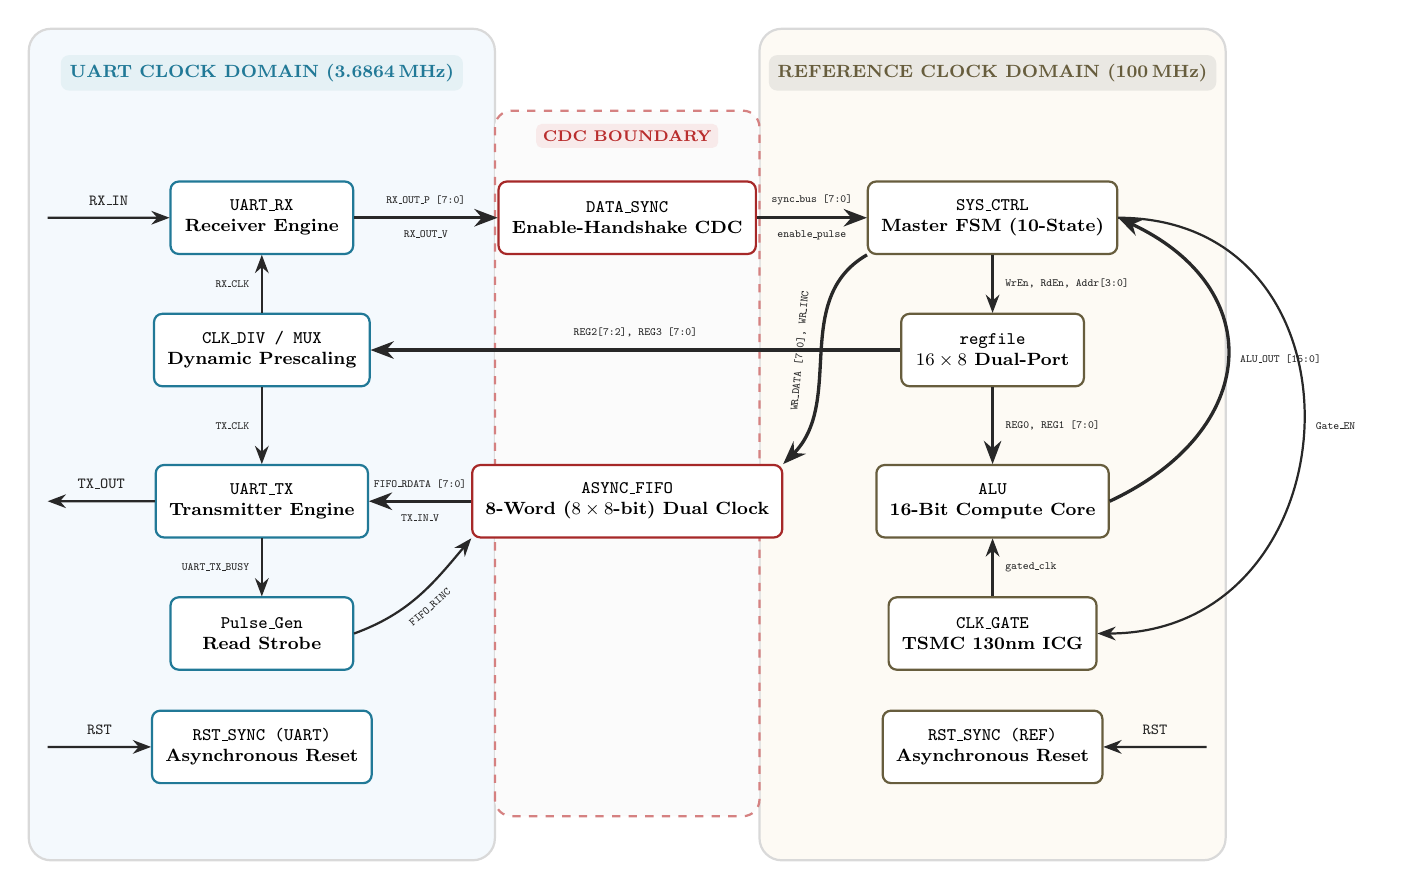
\begin{tikzpicture}[
    scale=0.80, transform shape,
    >=Stealth,
    uartblock/.style={draw=primary!90!black, thick, fill=white, rounded corners=3pt, align=center, font=\footnotesize\bfseries, inner sep=6pt, minimum height=1.15cm, minimum width=2.9cm},
    refblock/.style={draw=accent!90!black, thick, fill=white, rounded corners=3pt, align=center, font=\footnotesize\bfseries, inner sep=6pt, minimum height=1.15cm, minimum width=2.9cm},
    cdcblock/.style={draw=cdcalert!90!black, thick, fill=white, rounded corners=3pt, align=center, font=\footnotesize\bfseries, inner sep=6pt, minimum height=1.15cm, minimum width=3.3cm},
    domainbox/.style={draw=gray!30, thick, rounded corners=8pt, fill=#1},
    signal/.style={->, thick, darkcharcoal},
    bus/.style={->, very thick, darkcharcoal}
]

% Background Clock Domains
\node[domainbox=uartbg, minimum width=7.4cm, minimum height=13.2cm] at (-5.8, -0.9) {};
\node[fill=primary!12, text=primary!90!black, font=\bfseries\footnotesize, rounded corners=3pt, inner sep=4pt] at (-5.8, 5.0) {UART CLOCK DOMAIN (3.6864\,MHz)};

\node[domainbox=refbg, minimum width=7.4cm, minimum height=13.2cm] at (5.8, -0.9) {};
\node[fill=accent!15, text=accent!90!black, font=\bfseries\footnotesize, rounded corners=3pt, inner sep=4pt] at (5.8, 5.0) {REFERENCE CLOCK DOMAIN (100\,MHz)};

% CDC Boundary Region in Center
\draw[draw=cdcalert!60, dashed, thick, rounded corners=6pt, fill=bannerbg!40] (-2.1, -6.8) rectangle (2.1, 4.4);
\node[fill=cdcalert!10, text=cdcalert, font=\bfseries\scriptsize, rounded corners=2pt, inner sep=3pt, align=center] at (0, 4.0) {CDC BOUNDARY};

% ==================== UART DOMAIN MODULES ====================
\node[uartblock] (rx) at (-5.8, 2.7) {\texttt{UART\_RX}\\Receiver Engine};
\node[uartblock] (clkdiv) at (-5.8, 0.6) {\texttt{CLK\_DIV / MUX}\\Dynamic Prescaling};
\node[uartblock] (tx) at (-5.8, -1.8) {\texttt{UART\_TX}\\Transmitter Engine};
\node[uartblock] (pulse) at (-5.8, -3.9) {\texttt{Pulse\_Gen}\\Read Strobe};
\node[uartblock] (rst_uart) at (-5.8, -5.7) {\texttt{RST\_SYNC (UART)}\\Asynchronous Reset};

% ==================== CDC BOUNDARY MODULES ====================
\node[cdcblock] (datasync) at (0, 2.7) {\texttt{DATA\_SYNC}\\Enable-Handshake CDC};
\node[cdcblock] (fifo) at (0, -1.8) {\texttt{ASYNC\_FIFO}\\8-Word ($8\times 8$-bit) Dual Clock};

% ==================== REF DOMAIN MODULES ====================
\node[refblock] (fsm) at (5.8, 2.7) {\texttt{SYS\_CTRL}\\Master FSM (10-State)};
\node[refblock] (rf) at (5.8, 0.6) {\texttt{regfile}\\$16\times 8$ Dual-Port};
\node[refblock] (alu) at (5.8, -1.8) {\texttt{ALU}\\16-Bit Compute Core};
\node[refblock] (icg) at (5.8, -3.9) {\texttt{CLK\_GATE}\\TSMC 130nm ICG};
\node[refblock] (rst_ref) at (5.8, -5.7) {\texttt{RST\_SYNC (REF)}\\Asynchronous Reset};

% ==================== INTERCONNECT SIGNALS ====================

% RX_IN input to UART_RX
\draw[signal] (-9.2, 2.7) -- node[above=2pt, font=\scriptsize\bfseries] {\texttt{RX\_IN}} (rx.west);

% UART_RX to DATA_SYNC
\draw[bus] (rx.east) -- node[above=2pt, font=\tiny\bfseries] {\texttt{RX\_OUT\_P [7:0]}}
                        node[below=2pt, font=\tiny\bfseries] {\texttt{RX\_OUT\_V}} (datasync.west);

% DATA_SYNC to SYS_CTRL
\draw[bus] (datasync.east) -- node[above=2pt, font=\tiny\bfseries] {\texttt{sync\_bus [7:0]}}
                              node[below=2pt, font=\tiny\bfseries] {\texttt{enable\_pulse}} (fsm.west);

% SYS_CTRL to RegFile
\draw[signal] (fsm.south) -- node[right=2pt, font=\tiny\bfseries] {\texttt{WrEn, RdEn, Addr[3:0]}} (rf.north);

% RegFile to ALU
\draw[bus] (rf.south) -- node[right=2pt, font=\tiny\bfseries] {\texttt{REG0, REG1 [7:0]}} (alu.north);

% SYS_CTRL to CLK_GATE (Enable)
\draw[signal] (fsm.east) to[out=0, in=0, looseness=1.6] node[right=2pt, font=\tiny\bfseries] {\texttt{Gate\_EN}} (icg.east);

% CLK_GATE to ALU (Gated Clock)
\draw[signal] (icg.north) -- node[right=2pt, font=\tiny\bfseries] {\texttt{gated\_clk}} (alu.south);

% ALU output to SYS_CTRL (Feedback on right)
\draw[bus] (alu.east) to[out=25, in=335, looseness=1.5] node[right=2pt, font=\tiny\bfseries] {\texttt{ALU\_OUT [15:0]}} (fsm.east);

% SYS_CTRL to ASYNC_FIFO (Write Interface)
\draw[bus] (fsm.south west) to[out=210, in=45] node[above=3pt, sloped, font=\tiny\bfseries] {\texttt{WR\_DATA [7:0], WR\_INC}} (fifo.north east);

% RegFile to CLK_DIV (Baud & Prescale Configuration)
\draw[bus] (rf.west) -- node[above=2pt, font=\tiny\bfseries] {\texttt{REG2[7:2], REG3 [7:0]}} (clkdiv.east);

% CLK_DIV to RX and TX clocks
\draw[signal] (clkdiv.north) -- node[left=2pt, font=\tiny\bfseries] {\texttt{RX\_CLK}} (rx.south);
\draw[signal] (clkdiv.south) -- node[left=2pt, font=\tiny\bfseries] {\texttt{TX\_CLK}} (tx.north);

% ASYNC_FIFO to UART_TX (Read Interface)
\draw[bus] (fifo.west) -- node[above=2pt, font=\tiny\bfseries] {\texttt{FIFO\_RDATA [7:0]}}
                          node[below=2pt, font=\tiny\bfseries] {\texttt{TX\_IN\_V}} (tx.east);

% UART_TX output to TX_OUT
\draw[signal] (tx.west) -- node[above=2pt, font=\scriptsize\bfseries] {\texttt{TX\_OUT}} (-9.2, -1.8);

% UART_TX to Pulse_Gen (Busy Trigger)
\draw[signal] (tx.south) -- node[left=2pt, font=\tiny\bfseries] {\texttt{UART\_TX\_BUSY}} (pulse.north);

% Pulse_Gen to ASYNC_FIFO (Read Increment)
\draw[signal] (pulse.east) to[out=20, in=230] node[below=2pt, sloped, font=\tiny\bfseries] {\texttt{FIFO\_RINC}} (fifo.south west);

% Global Reset Inputs
\draw[signal] (-9.2, -5.7) -- node[above=2pt, font=\scriptsize\bfseries] {\texttt{RST}} (rst_uart.west);
\draw[signal] (9.2, -5.7) -- node[above=2pt, font=\scriptsize\bfseries] {\texttt{RST}} (rst_ref.east);

\end{tikzpicture}
}
\caption{System Architecture showing clock domain partitioning, CDC synchronization boundaries, and internal bus interconnect.}
\label{fig:sys_arch}
\end{figure}

\begin{table}[H]
\centering
\caption{System Clock Domains, Frequencies, and Synchronized Reset Mapping.}
\label{tab:clock_domains}
\renewcommand{\arraystretch}{1.3}
\begin{tabularx}{\textwidth}{|Y|Y|Y|Y|Y|}
\hline
\textbf{Domain Name} & \textbf{Source Clock} & \textbf{Frequency} & \textbf{Reset Domain} & \textbf{Hosted Subsystems} \\
\hline
\textbf{Reference Domain} & \texttt{REF\_CLK} & 100\,MHz & \texttt{REF\_RST} & \texttt{SYS\_CTRL}, \texttt{regfile}, \texttt{ALU}, \texttt{CLK\_GATE}, FIFO Write Port \\
\hline
\textbf{UART Serial Domain} & \texttt{UART\_CLK} & 3.6864\,MHz & \texttt{UART\_RST} & \texttt{UART\_RX}, \texttt{UART\_TX}, \texttt{CLK\_DIV}, \texttt{Pulse\_}\allowbreak\texttt{Gen}, FIFO Read Port \\
\hline
\textbf{Gated Compute Domain} & \texttt{gated\_clk} & 0--100\,MHz & \texttt{REF\_RST} & 16-Bit Arithmetic Core (Internal ALU Switching Logic) \\
\hline
\end{tabularx}
\vspace{2pt}
{\footnotesize\textit{Note}: the FIFO read port and \texttt{Pulse\_Gen} are clocked by \texttt{TX\_CLK} (\texttt{UART\_CLK} $\div$ 32 baud clock).}
\end{table}

% ------------------------------------------------------------------------------
% SECTION 3: CDC SYNCHRONIZATION ARCHITECTURE
% ------------------------------------------------------------------------------
\section{Comprehensive Clock Domain Crossing (CDC) Synchronization}

\subsection{Theoretical Foundations: Metastability and Multi-Bit Skew Hazards}
When a digital signal transitions asynchronously with respect to the sampling clock of a destination register, setup ($t_{\text{su}}$) or hold ($t_h$) timing margins may be violated. The destination flip-flop's internal bistable feedback loop enters a metastable state where its output voltage hovers indeterminately between logical 0 and 1 for an unbounded settling duration. The probability of failure is quantified by the Mean Time Between Failures (MTBF)~\cite{cummings_cdc}:

\begin{equation}
\text{MTBF} = \frac{e^{\frac{t_r}{\tau}}}{T_0 \cdot f_{\text{clk}} \cdot f_{\text{data}}}
\end{equation}
where $t_r$ is the resolving time margin, $\tau$ is the flip-flop regenerative time constant, $T_0$ is an asymptotic thermal factor, $f_{\text{clk}}$ is the destination clock frequency, and $f_{\text{data}}$ is the asynchronous data transition frequency.

While a single-bit control signal can be protected using a two-stage flip-flop synchronizer, \textbf{multi-bit buses cannot be synchronized by placing individual synchronizers on each data line}. Due to non-uniform interconnect routing delays, process variations, and parasitic wire capacitance, individual bits experience unequal skew. If the bus transitions during the destination clock edge, certain bits will resolve in destination cycle $N$ while others resolve in cycle $N+1$, resulting in catastrophic \textbf{bus incoherency} (capturing corrupted, blended data words).

To eliminate metastability and bus incoherency, the system implements three specialized CDC circuits:

\subsection{Multi-Bit Data Synchronizer (\texttt{DATA\_SYNC})}

\subsubsection{Architectural Function \& Mechanics}
The \texttt{DATA\_SYNC} module safely transfers the received 8-bit parallel byte (\texttt{RX\_OUT\_P}) and valid flag (\texttt{RX\_OUT\_V}) from the slow 3.6864\,MHz \texttt{UART\_CLK} domain into the high-speed 100\,MHz \texttt{REF\_CLK} domain. It employs an \textbf{enable-handshake synchronization topology}:
\begin{enumerate}
    \item The 8-bit data bus (\texttt{RX\_OUT\_P}) is driven statically by the UART receiver and held constant while the transfer occurs.
    \item The single-bit valid strobe (\texttt{RX\_OUT\_V}) is routed into the synchronizer as \texttt{bus\_enable} and passed through a 2-stage flip-flop synchronizer clocked by \texttt{REF\_CLK}.
    \item An edge-detector flip-flop generates a single-cycle pulse (\texttt{enable\_pulse}) in the \texttt{REF\_CLK} domain when the synchronized enable rises:
    \begin{equation}
    \texttt{pulse\_gen\_out} = \texttt{multi\_flops}[1] \;\land\; \neg\texttt{enable\_flop}
    \end{equation}
    \item On \texttt{pulse\_gen\_out}, a multiplexer updates \texttt{sync\_bus} with \texttt{unsync\_bus}, latching the fully settled data bus into the destination domain registers.
\end{enumerate}

\subsubsection{Design Rationale: Why We Used It (Problem Solved)}
Without \texttt{DATA\_SYNC}, passing an 8-bit received byte directly across the clock boundary would cause multi-bit skew incoherency. An alternative approach would be to instantiate a full dual-clock FIFO at the receiver output. However, because UART frames arrive at a maximum rate of 11,520 bytes/second ($\approx 86.8\,\mu\text{s}$ per byte), the destination 100\,MHz FSM consumes each byte in tens of nanoseconds. There is zero risk of back-to-back byte collision. Therefore, an enable-handshake synchronizer solves the multi-bit CDC hazard with complete coherency while requiring a fraction of the silicon area of a FIFO.

\subsubsection{Key Engineering Benefits}
\begin{itemize}
    \item \textbf{100\% Bus Coherency}: The multi-bit data lines never transition during the sampling window; only the synchronized control pulse triggers sampling.
    \item \textbf{Silicon Area Efficiency}: Consumes only 3 control flip-flops, 8 data register bits, and minimal gating logic ($\approx 404\,\mu\text{m}^2$ synthesized, \texttt{U0\_DATA\_SYNC}) compared to $\approx 4{,}103\,\mu\text{m}^2$ for the asynchronous FIFO (\texttt{U0\_ASYNC\_FIFO}).
    \item \textbf{Deterministic Handshake}: Produces an exact 1-clock-cycle \texttt{enable\_pulse} that directly drives the FSM state transition logic without race conditions.
\end{itemize}

\begin{lstlisting}[caption={RTL Implementation of the Multi-Bit Data Synchronizer (DATA\_SYNC.v).}]
module DATA_SYNC #(parameter bus_width = 8, stages = 2) (
    input  wire                     clk, rst, bus_enable,
    input  wire [bus_width - 1 : 0] unsync_bus,
    output reg  [bus_width - 1 : 0] sync_bus,
    output reg                      enable_pulse
);
  reg [0 : stages - 1] multi_flops;
  reg                  enable_flop;
  wire                 pulse_gen_out;
  wire [bus_width-1:0] mux_out;

  // Multi-stage flip-flop synchronizer on bus_enable control strobe
  always @(posedge clk or negedge rst) begin
    if (!rst) multi_flops <= 'b0;
    else      multi_flops <= {bus_enable, multi_flops[0 : stages - 2]};
  end

  // Edge-detector flop for single-cycle pulse generation
  always @(posedge clk or negedge rst) begin
    if (!rst) enable_flop <= 1'b0;
    else      enable_flop <= multi_flops[stages-1];
  end

  assign pulse_gen_out = multi_flops[stages-1] && !enable_flop;
  assign mux_out       = pulse_gen_out ? unsync_bus : sync_bus;

  // Register coherent data bus on synchronized enable pulse
  always @(posedge clk or negedge rst) begin
    if (!rst) begin
      sync_bus     <= 'b0;
      enable_pulse <= 1'b0;
    end else begin
      sync_bus     <= mux_out;
      enable_pulse <= pulse_gen_out;
    end
  end
endmodule
\end{lstlisting}

\subsection{Dual-Clock Asynchronous FIFO (\texttt{ASYNC\_FIFO})}

\subsubsection{Architectural Function \& Mechanics}
The \texttt{ASYNC\_FIFO} bridges the high-speed \texttt{REF\_CLK} domain (write side) and the slow \texttt{UART\_CLK} domain (read side). When the 16-bit ALU produces execution results or the Register File performs a memory read, the 8-bit bytes are written into the FIFO. The UART transmitter autonomously reads these bytes and serializes them. The module comprises five sub-blocks (Figure~\ref{fig:fifo_arch}):
\begin{itemize}
    \item \texttt{FIFO\_MEM\_CNTRL}: An $8\times 8$-bit dual-port static register array with synchronous write on \texttt{wclk} and combinational read on \texttt{raddr}.
    \item \texttt{FIFO\_WR}: Write address counter and full flag generator operating strictly in \texttt{wclk}.
    \item \texttt{FIFO\_RD}: Read address counter and empty flag generator operating strictly in \texttt{rclk}.
    \item \texttt{DF\_SYNC (Write-to-Read)}: Synchronizes the 4-bit Gray write pointer (\texttt{wptr\_gray}) into the read clock domain (\texttt{rq2\_wptr}).
    \item \texttt{DF\_SYNC (Read-to-Write)}: Synchronizes the 4-bit Gray read pointer (\texttt{rptr\_gray}) into the write clock domain (\texttt{wq2\_rptr}).
\end{itemize}

\begin{figure}[H]
\centering
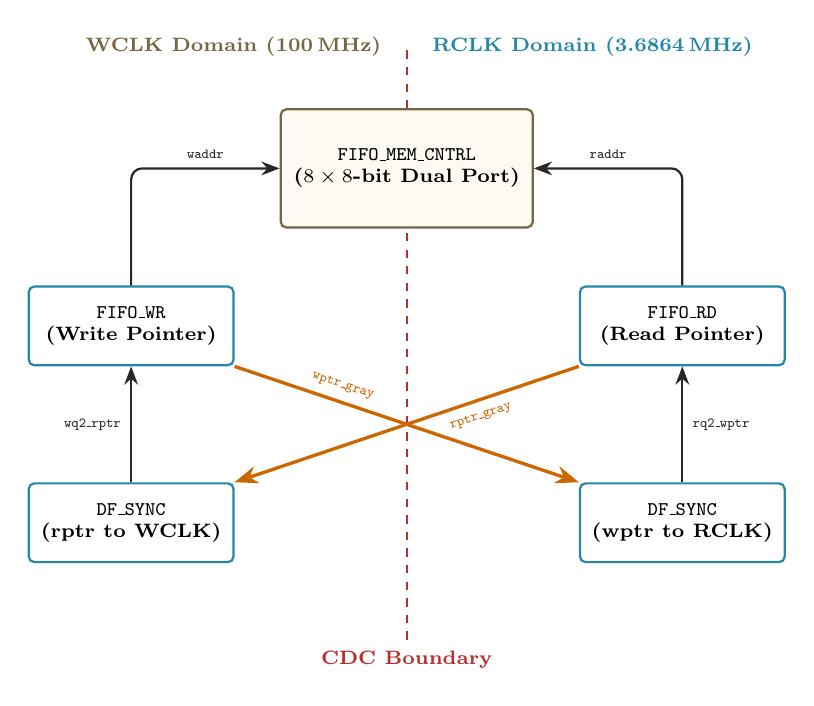
\begin{tikzpicture}[
    >=Stealth,
    block/.style={draw=primary, thick, fill=white, rounded corners=2pt, align=center, font=\scriptsize\bfseries, minimum width=2.6cm, minimum height=1cm},
    mem/.style={draw=accent, thick, fill=refbg, rounded corners=2pt, align=center, font=\scriptsize\bfseries, minimum width=3.2cm, minimum height=1.5cm},
    arrow/.style={->, thick, darkcharcoal}
]
    % Domains Boundary
    \draw[dashed, cdcalert, thick] (0, 3) -- (0, -4.5) node[below, font=\scriptsize\bfseries] {CDC Boundary};
    \node[anchor=south east, font=\scriptsize\bfseries, text=accent] at (-0.2, 2.8) {WCLK Domain (100\,MHz)};
    \node[anchor=south west, font=\scriptsize\bfseries, text=primary] at (0.2, 2.8) {RCLK Domain (3.6864\,MHz)};

    % Memory Array
    \node[mem] (mem) at (0, 1.5) {\texttt{FIFO\_MEM\_CNTRL}\\($8 \times 8$-bit Dual Port)};

    % Write & Read Controllers
    \node[block] (wr) at (-3.5, -0.5) {\texttt{FIFO\_WR}\\(Write Pointer)};
    \node[block] (rd) at (3.5, -0.5) {\texttt{FIFO\_RD}\\(Read Pointer)};

    % Synchronizers (Crossed Domains)
    \node[block] (syncW) at (3.5, -3) {\texttt{DF\_SYNC}\\(wptr to RCLK)};
    \node[block] (syncR) at (-3.5, -3) {\texttt{DF\_SYNC}\\(rptr to WCLK)};

    % Memory Connections
    \draw[arrow, rounded corners] (wr.north) |- node[above, near end, font=\tiny] {\texttt{waddr}} (mem.west);
    \draw[arrow, rounded corners] (rd.north) |- node[above, near end, font=\tiny] {\texttt{raddr}} (mem.east);

    % Synchronized Pointers Return (Upwards straight to blocks)
    \draw[arrow] (syncW.north) -- node[right, font=\tiny] {\texttt{rq2\_wptr}} (rd.south);
    \draw[arrow] (syncR.north) -- node[left, font=\tiny] {\texttt{wq2\_rptr}} (wr.south);

    % Gray Code Crossing (highlighted: Gray-code pointer synchronization)
    \definecolor{grayptr}{RGB}{204,102,0}
    \draw[arrow, very thick, grayptr] (wr.south east) -- node[above, sloped, pos=0.3, font=\tiny, text=grayptr] {\texttt{wptr\_gray}} (syncW.north west);
    \draw[arrow, very thick, grayptr] (rd.south west) -- node[below, sloped, pos=0.3, font=\tiny, text=grayptr] {\texttt{rptr\_gray}} (syncR.north east);

\end{tikzpicture}
\caption{ASYNC\_FIFO Architecture highlighting Gray-Code Pointer Synchronization.}
\label{fig:fifo_arch}
\end{figure}

\subsubsection{Design Rationale: Why We Used It (Problem Solved)}
The ALU and System Controller generate 16-bit results as two consecutive bytes in back-to-back 100\,MHz clock cycles (20\,ns total). Conversely, transmitting a single UART byte at 115,200 baud requires $86.8\,\mu\text{s}$ ($\approx 8,680$ reference clock cycles). Without an elastic asynchronous FIFO buffer, the 100\,MHz master processor would be forced to enter hard stall states for thousands of cycles waiting for each serial byte to transmit, crippling system computational throughput. The FIFO absorbs burst ALU and Register read responses instantaneously, completely decoupling compute performance from serial line latency.

\subsubsection{Why Gray-Coded Pointers Are Mandatory}
In standard binary counters, incrementing an address frequently causes multiple bits to toggle simultaneously (for example, transition $0111_2 \to 1000_2$ flips all 4 bits). When these bits pass across asynchronous clock boundaries, unequal wire delays and flip-flop setup characteristics cause the destination domain to capture transient, erroneous intermediate words (such as $1111_2$), falsely triggering full or empty flags and corrupting data pointers.

Gray code guarantees that \textbf{exactly one bit changes per address increment}:
\begin{equation}
\text{Gray\_Next} = \text{Bin\_Next} \;\oplus\; (\text{Bin\_Next} \mathbin{>>} 1)
\end{equation}
If the destination clock edge arrives precisely during a pointer bit transition, that bit may resolve to either its previous value or its new value. Because only one bit is changing, the captured Gray pointer is guaranteed to be either the old pointer value or the new pointer value---\textbf{never an arbitrary, illegal intermediate state}. If it resolves to the old pointer, the FIFO simply defers a full or empty release by one cycle, maintaining absolute data integrity.

\subsubsection{Cummings' Full and Empty Detection Formulation}
The FIFO utilizes $(N+1)$-bit pointers for a $2^N$-deep memory array ($N=3$, depth = 8 words)~\cite{cummings_fifo}. The $(N+1)$-th bit distinguishes between an empty buffer and a full buffer:
\begin{itemize}
    \item \textbf{FIFO Empty Condition} (Evaluated strictly in \texttt{rclk} domain):
    \begin{equation}
    \texttt{rempty} = (\texttt{rq2\_wptr} == \texttt{rptr\_gray\_reg})
    \end{equation}
    \item \textbf{FIFO Full Condition} (Evaluated strictly in \texttt{wclk} domain): The write pointer has wrapped around exactly once and caught up with the synchronized read pointer. In Gray code, this condition is met when the two MSBs are inverted while all lower bits match:
    \begin{equation}
    \begin{split}
    \texttt{wfull} = & (\texttt{wq2\_rptr}[3] \neq \texttt{wgray}[3]) \;\land\; (\texttt{wq2\_rptr}[2] \neq \texttt{wgray}[2]) \\
                     & \;\land\; (\texttt{wq2\_rptr}[1:0] == \texttt{wgray}[1:0])
    \end{split}
    \end{equation}
\end{itemize}

\begin{lstlisting}[caption={Write Pointer and Full Flag Generation (FIFO\_WR.v).}]
module FIFO_WR(
    input  wire       winc, wrst_n, wclk,
    input  wire [3:0] wq2_rptr,
    output wire [2:0] waddr,
    output wire [3:0] wptr_gray,
    output wire       wfull
);
  reg [3:0] wcounter, wptr_gray_reg;
  reg       wfull_reg;

  wire [3:0] wcounter_next      = (winc && !wfull_reg) ? wcounter + 4'd1 : wcounter;
  wire [3:0] wcounter_gray_next = wcounter_next ^ (wcounter_next >> 1'b1);

  always @(posedge wclk or negedge wrst_n) begin
    if (!wrst_n) begin
      wcounter      <= 4'b0;
      wptr_gray_reg <= 4'b0;
      wfull_reg     <= 1'b0;
    end else begin
      wcounter      <= wcounter_next;
      wptr_gray_reg <= wcounter_gray_next;
      // Cummings Gray-code full condition: top two MSBs inverted, lower bits equal
      if ((wq2_rptr[3]   != wcounter_gray_next[3]) &&
          (wq2_rptr[2]   != wcounter_gray_next[2]) &&
          (wq2_rptr[1:0] == wcounter_gray_next[1:0]))
        wfull_reg <= 1'b1;
      else
        wfull_reg <= 1'b0;
    end
  end
  assign wptr_gray = wptr_gray_reg;
  assign waddr     = wcounter[2:0];
  assign wfull     = wfull_reg;
endmodule
\end{lstlisting}

\subsection{Dual-Domain Asynchronous Reset Synchronizers (\texttt{RST\_SYNC})}

\subsubsection{Architectural Function \& Mechanics}
The chip features an active-low global reset input (\texttt{RST}). Because this reset drives flip-flops in two asynchronous clock domains (\texttt{REF\_CLK} and \texttt{UART\_CLK}), two independent reset synchronizers are instantiated. Each synchronizer consists of a cascade of flip-flops configured with asynchronous reset pins tied to the external \texttt{RST} and data inputs tied to logic 1 (\texttt{VDD}).

\subsubsection{Design Rationale: Why We Used It (Problem Solved)}
Reset design involves an inherent dilemma:
\begin{itemize}
    \item \textbf{Pure Synchronous Reset}: Cannot reset the chip if the external clock oscillator is dead, unstable, or delayed during initial power-up.
    \item \textbf{Pure Asynchronous Reset}: When released asynchronously, if the deasserting reset edge falls within the setup/hold window of the clock edge, it violates flip-flop recovery time ($t_{\text{rec}}$) or removal time ($t_{\text{rem}}$). This causes random flip-flops to exit reset on clock cycle $N$ while adjacent flip-flops exit on cycle $N+1$, throwing state machines into illegal, deadlocked states.
\end{itemize}
The \texttt{RST\_SYNC} topology implements \textbf{Asynchronous Assertion with Synchronous Deassertion}~\cite{cummings_reset}:
\begin{enumerate}
    \item When \texttt{RST} drops low, all flip-flops assert reset \textbf{instantaneously} via their asynchronous clear pins, without waiting for clock edges.
    \item When \texttt{RST} goes high, the logic 1 on the D-input shifts through the multi-stage flop chain, releasing reset \textbf{synchronously} aligned to the local clock edge, completely eliminating recovery/removal violations.
\end{enumerate}

\begin{lstlisting}[caption={RTL Implementation of the Reset Synchronizer (RST\_SYNC.v).}]
module RST_SYNC #(parameter stages = 3) (
    input  wire rst, clk,
    output wire sync_rst
);
  reg [0 : stages - 1] flops;

  always @(posedge clk or negedge rst) begin
    if (!rst)
      flops <= 'b0;                               // Instantaneous asynchronous assertion
    else
      flops <= {1'b1, flops[0 : stages - 2]};     // Synchronous deassertion on clock edge
  end
  assign sync_rst = flops[stages-1];
endmodule
\end{lstlisting}

% ------------------------------------------------------------------------------
% SECTION 4: MASTER COMMUNICATION PROTOCOL & FRAME FORMATS
% ------------------------------------------------------------------------------
\section{Master Communication Protocol and Frame Formats}

\subsection{UART Serial Frame Specification}
Communication between the external host and the SoC occurs over a full-duplex, asynchronous serial link. Each serial frame consists of 10 or 11 bits depending on dynamic parity configuration:
\begin{itemize}
    \item \textbf{Start Bit}: 1 low bit (\texttt{1'b0}) indicating frame transmission start.
    \item \textbf{Data Payload}: 8 data bits transmitted strictly \textbf{Least Significant Bit (LSB) first}.
    \item \textbf{Parity Bit (Configurable)}: 1 bit enabled via \texttt{REG2[0]} with Even (\texttt{REG2[1]=0}) or Odd (\texttt{REG2[1]=1}) parity.
    \item \textbf{Stop Bit}: 1 high bit (\texttt{1'b1}) verifying framing integrity.
\end{itemize}

\subsection{Baud Rate and Oversampling Calculations}
Transmitter baud timing and receiver oversampling are synthesized directly from \texttt{UART\_CLK} ($3.6864\,\text{MHz}$) using programmable integer division ratios:
\begin{equation}
\text{TX Baud Rate} = \frac{f_{\text{UART\_CLK}}}{\text{TX Divisor (\texttt{REG3})}} = \frac{3,686,400\,\text{Hz}}{32} = 115,200\,\text{Baud}
\end{equation}

For the receiver, an oversampling factor ($M \in \{8, 16, 32\}$) is configured in \texttt{REG2[7:2]}. The prescaler multiplexer translates this into an integer divider ratio for \texttt{CLK\_DIV}:
\begin{equation}
f_{\text{RX\_CLK}} = \frac{f_{\text{UART\_CLK}}}{\text{Prescale Mux Ratio}} = 115,200 \times M
\end{equation}

\subsection{Master System Command Set}
The master controller executes four primary multi-byte command sequences, detailed in Table~\ref{tab:commands}.

\begin{table}[H]
\centering
\caption{System Command Set and Protocol Definitions.}
\label{tab:commands}
\renewcommand{\arraystretch}{1.3}
\begin{tabularx}{\textwidth}{|l|c|c|c|Y|}
\hline
\textbf{Command} & \textbf{Opcode} & \textbf{RX Bytes} & \textbf{TX Bytes} & \textbf{Functional Operation Sequence} \\
\hline
\textbf{RF Write}       & \texttt{0xAA} & 3 & 0 & [Opcode $\to$ Address $\to$ Data]. Writes 8-bit data into register \texttt{0x0}--\texttt{0xF}. \\
\hline
\textbf{RF Read}        & \texttt{0xBB} & 2 & 1 & [Opcode $\to$ Address]. Reads addressed register; SoC pushes data to FIFO $\to$ \texttt{UART\_TX}. \\
\hline
\textbf{ALU with Op}    & \texttt{0xCC} & 4 & 2 & [Opcode $\to$ Op A $\to$ Op B $\to$ ALU FUN]. Writes \texttt{REG0}, \texttt{REG1}, executes ALU, pushes 16-bit result (MSB then LSB) to FIFO. \\
\hline
\textbf{ALU without Op} & \texttt{0xDD} & 2 & 2 & [Opcode $\to$ ALU FUN]. Executes ALU on cached \texttt{REG0}, \texttt{REG1}; pushes 16-bit result (MSB then LSB) to FIFO. \\
\hline
\end{tabularx}
\end{table}

% ------------------------------------------------------------------------------
% SECTION 5: DETAILED SUBSYSTEM HARDWARE ARCHITECTURE
% ------------------------------------------------------------------------------
\section{Detailed Subsystem Hardware Architecture}

\subsection{System Controller (\texttt{SYS\_CTRL})}

\begin{figure}[H]
\centering
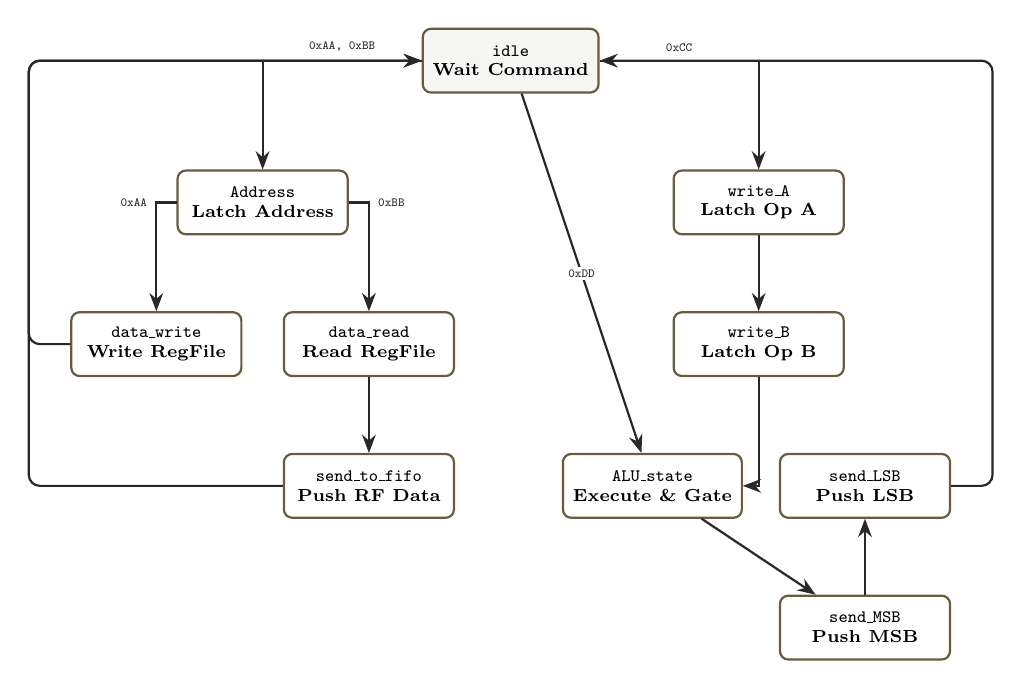
\begin{tikzpicture}[
    scale=0.9, transform shape,
    >=Stealth,
    state/.style={draw=accent!90!black, thick, rounded corners=3pt, fill=white, align=center, font=\scriptsize\bfseries, inner sep=4pt, minimum height=0.9cm, minimum width=2.4cm},
    arrow/.style={->, thick, darkcharcoal}
]
    \node[state, fill=bannerbg] (idle) at (0, 4.5) {\texttt{idle}\\Wait Command};

    % Left Branch (0xAA, 0xBB)
    \node[state] (addr) at (-3.5, 2.5) {\texttt{Address}\\Latch Address};
    \node[state] (wr) at (-5.0, 0.5) {\texttt{data\_write}\\Write RegFile};
    \node[state] (rd) at (-2.0, 0.5) {\texttt{data\_read}\\Read RegFile};
    \node[state] (fifo_rd) at (-2.0, -1.5) {\texttt{send\_to\_fifo}\\Push RF Data};

    % Right Branch (0xCC)
    \node[state] (wr_a) at (3.5, 2.5) {\texttt{write\_A}\\Latch Op A};
    \node[state] (wr_b) at (3.5, 0.5) {\texttt{write\_B}\\Latch Op B};
    \node[state] (alu) at (2.0, -1.5) {\texttt{ALU\_state}\\Execute \& Gate};
    \node[state] (lsb) at (5.0, -1.5) {\texttt{send\_LSB}\\Push LSB};
    \node[state] (msb) at (5.0, -3.5) {\texttt{send\_MSB}\\Push MSB};

    % Transitions Forward
    \draw[arrow] (idle) -| node[above, near start, font=\tiny] {\texttt{0xAA, 0xBB}} (addr);
    \draw[arrow] (addr) -| node[left, font=\tiny] {\texttt{0xAA}} (wr);
    \draw[arrow] (addr) -| node[right, font=\tiny] {\texttt{0xBB}} (rd);
    \draw[arrow] (rd) -- (fifo_rd);

    \draw[arrow] (idle) -| node[above, near start, font=\tiny] {\texttt{0xCC}} (wr_a);
    \draw[arrow] (idle) -- node[fill=white, inner sep=1pt, font=\tiny] {\texttt{0xDD}} (alu);
    \draw[arrow] (wr_a) -- (wr_b);
    \draw[arrow] (wr_b) |- (alu);
    \draw[arrow] (alu) -- (msb);
    \draw[arrow] (msb) -- (lsb);

    % Clean Return Lines to Idle (Outer Routing)
    \draw[arrow, rounded corners=4pt] (wr.west) -- (-6.8, 0.5) |- (idle.west);
    \draw[arrow, rounded corners=4pt] (fifo_rd.west) -- (-6.8, -1.5) |- (idle.west);
    \draw[arrow, rounded corners=4pt] (lsb.east) -- (6.8, -1.5) |- (idle.east);

\end{tikzpicture}
\caption{System Controller Finite State Machine state transition flow.}
\label{fig:fsm_states}
\end{figure}

\subsubsection{Architectural Function \& Mechanics}
Operating in the \texttt{REF\_CLK} domain, \texttt{SYS\_CTRL} acts as the master coordinator finite state machine. It contains 10 states: \texttt{idle}, \texttt{Address}, \texttt{data\_write}, \texttt{data\_read}, \texttt{send\_to\_fifo}, \texttt{write\_A}, \texttt{write\_B}, \texttt{ALU\_state}, \texttt{send\_LSB}, and \texttt{send\_MSB} (Figure~\ref{fig:fsm_states}).

\subsubsection{Design Rationale: Why We Used It (Problem Solved)}
Serial commands arrive sequentially over thousands of clock cycles. A centralized FSM is mandatory to enforce strict multi-byte protocol framing, route incoming data into the appropriate internal destinations, manage register access strobes (\texttt{WrEn}, \texttt{RdEn}), dynamically assert ALU clock gate enables (\texttt{Gate\_EN}), and sequence 16-bit split-byte pushes into the FIFO.

\subsubsection{Key Engineering Benefits}
\begin{itemize}
    \item \textbf{Deterministic Protocol Sequencing}: Implements unambiguous multi-byte state handling that rejects malformed commands.
    \item \textbf{Atomic Multi-Byte Operations}: Automatically splits 16-bit ALU outputs into ordered MSB-then-LSB byte transfers.
    \item \textbf{Autonomous Power Management}: Directly asserts \texttt{Gate\_EN} strictly during active computational states.
\end{itemize}

\subsection{Register File (\texttt{regfile})}

\subsubsection{Architectural Function \& Mechanics}
The Register File provides 16 directly addressable 8-bit registers ($128$ bits total storage). It features separate write and read ports:
\begin{itemize}
    \item \texttt{REG0} (Address \texttt{0x0}): Dedicated Operand A for the 16-bit ALU.
    \item \texttt{REG1} (Address \texttt{0x1}): Dedicated Operand B for the 16-bit ALU.
    \item \texttt{REG2} (Address \texttt{0x2}): UART Configuration: \texttt{REG2[0]} (Parity Enable), \texttt{REG2[1]} (Parity Type: 0=Even, 1=Odd), \texttt{REG2[7:2]} (Prescaler Division Ratio).
    \item \texttt{REG3} (Address \texttt{0x3}): Transmitter Baud Division Ratio (default value: $32$ for 115,200 Baud).
    \item \texttt{REG4}--\texttt{REG15} (Addresses \texttt{0x4}--\texttt{0xF}): General-purpose storage registers for user application data.
\end{itemize}

\subsubsection{Design Rationale: Why We Used It (Problem Solved)}
Without a centralized register file, peripheral configuration parameters (baud rate, parity mode, prescaler ratios) would have to be hardwired at synthesis, eliminating operational flexibility. The Register File memory-maps peripheral control, enabling software to dynamically alter communication parameters at runtime while providing dedicated zero-wait-state ports directly into the ALU.

\subsubsection{Key Engineering Benefits}
\begin{itemize}
    \item \textbf{Zero-Cycle Read Latency}: Provides instantaneous combinational operand delivery to the ALU.
    \item \textbf{Run-Time Peripheral Reconfigurability}: Allows on-the-fly baud rate and parity tuning via standard UART commands.
    \item \textbf{Dedicated Port Isolation}: Prevents ALU data fetches from contending with serial host register accesses.
\end{itemize}

\subsection{16-Bit Arithmetic Logic Unit (\texttt{ALU})}

\subsubsection{Architectural Function \& Mechanics}
The ALU operates on two 8-bit operands (\texttt{A} and \texttt{B}) and yields a full-precision 16-bit output (\texttt{ALU\_OUT}) alongside an output valid strobe (\texttt{out\_valid}). It supports 16 distinct operations grouped into four categories, summarized in Table~\ref{tab:alu_ops}.

\begin{table}[H]
\centering
\caption{ALU Function Opcode Mapping.}
\label{tab:alu_ops}
\renewcommand{\arraystretch}{1.25}
\begin{tabularx}{\textwidth}{|l|c|l|Y|}
\hline
\textbf{Category} & \textbf{ALU\_FUN} & \textbf{Operation} & \textbf{Mathematical Description} \\
\hline
\multirow{4}{*}{\textbf{Arithmetic}}
 & \texttt{4'b0000} & Addition       & $\text{ALU\_OUT} = A + B$ \\ \cline{2-4}
 & \texttt{4'b0001} & Subtraction    & $\text{ALU\_OUT} = A - B$ \\ \cline{2-4}
 & \texttt{4'b0010} & Multiplication & $\text{ALU\_OUT} = A \times B$ ($8\times 8 \to 16$-bit full precision) \\ \cline{2-4}
 & \texttt{4'b0011} & Division       & $\text{ALU\_OUT} = A / B$ (returns \texttt{16'd0} when $B=0$) \\
\hline
\multirow{6}{*}{\textbf{Logical}}
 & \texttt{4'b0100} & Bitwise AND    & $\text{ALU\_OUT} = \{\texttt{8'b0}, A \;\land\; B\}$ \\ \cline{2-4}
 & \texttt{4'b0101} & Bitwise OR     & $\text{ALU\_OUT} = \{\texttt{8'b0}, A \;\lor\; B\}$ \\ \cline{2-4}
 & \texttt{4'b0110} & Bitwise NAND   & $\text{ALU\_OUT} = \{\texttt{8'b0}, \neg(A \;\land\; B)\}$ \\ \cline{2-4}
 & \texttt{4'b0111} & Bitwise NOR    & $\text{ALU\_OUT} = \{\texttt{8'b0}, \neg(A \;\lor\; B)\}$ \\ \cline{2-4}
 & \texttt{4'b1000} & Bitwise XOR    & $\text{ALU\_OUT} = \{\texttt{8'b0}, A \;\oplus\; B\}$ \\ \cline{2-4}
 & \texttt{4'b1001} & Bitwise XNOR   & $\text{ALU\_OUT} = \{\texttt{8'b0}, \neg(A \;\oplus\; B)\}$ \\
\hline
\multirow{3}{*}{\textbf{Comparison}}
 & \texttt{4'b1010} & Equality       & $\text{ALU\_OUT} = (A == B) \;?\; \texttt{16'd1} : \texttt{16'd0}$ \\ \cline{2-4}
 & \texttt{4'b1011} & Greater Than   & $\text{ALU\_OUT} = (A > B) \;?\; \texttt{16'd2} : \texttt{16'd0}$ \\ \cline{2-4}
 & \texttt{4'b1100} & Less Than      & $\text{ALU\_OUT} = (A < B) \;?\; \texttt{16'd3} : \texttt{16'd0}$ \\
\hline
\multirow{3}{*}{\textbf{Shift / Pass}}
 & \texttt{4'b1101} & Shift Right    & $\text{ALU\_OUT} = \{\texttt{8'b0}, A \mathbin{>>} 1\}$ \\ \cline{2-4}
 & \texttt{4'b1110} & Shift Left     & $\text{ALU\_OUT} = \{\texttt{8'b0}, A \mathbin{<<} 1\}$ \\ \cline{2-4}
 & \texttt{4'b1111} & Reserved (default) & Unused encoding --- output forced to \texttt{16'd0} and \texttt{out\_valid} cleared \\
\hline
\end{tabularx}
\end{table}

\subsubsection{Design Rationale: Why We Used It (Problem Solved)}
The 16-bit ALU serves as the primary hardware accelerator. Dedicated 16-bit output width eliminates numerical truncation and overflow hazards during arithmetic addition and multiplication, returning complete 16-bit mathematical precision to the host computer.

\subsubsection{Key Engineering Benefits}
\begin{itemize}
    \item \textbf{Single-Cycle Combinational Execution}: Produces full 16-bit arithmetic and logical results in 1 clock cycle.
    \item \textbf{Zero Overflow Hazard}: 16-bit output accommodates the maximum product of two 8-bit numbers ($255 \times 255 = 65,025$).
    \item \textbf{Gated Clocking Interface}: Fully isolated by the clock gating subsystem, drawing near-zero dynamic power when unselected.
\end{itemize}

\subsection{Integrated Clock Gating Cell (\texttt{CLK\_GATE})}

\subsubsection{Architectural Function \& Mechanics}
The \texttt{CLK\_GATE} module implements latch-based clock gating. In synthesis mode (\texttt{SYNTHESIS=1}), it instantiates the TSMC 130nm library cell \texttt{TLATNCAX2M}. In behavioral simulation mode (\texttt{SYNTHESIS=0}), it evaluates an active-low transparent latch driving an AND gate:
\begin{equation}
\texttt{gated\_clk} = \texttt{clk} \;\land\; \texttt{latch}
\end{equation}

\subsubsection{Design Rationale: Why Latch-Based ICG Is Mandatory vs. Simple AND Gate}
A common misconception in digital design is gating a clock tree using a simple 2-input AND gate between \texttt{clk} and \texttt{clk\_en}. \textbf{A simple AND gate produces catastrophic clock glitches}: if \texttt{clk\_en} transitions from 0 to 1 while \texttt{clk} is high, the output generates an immediate, truncated narrow clock pulse. This narrow glitch violates the minimum pulse-width requirement of destination flip-flops, causing unpredictable state corruption.

The active-low latch solves this hazard:
\begin{enumerate}
    \item When \texttt{clk} is LOW, the latch is transparent, allowing \texttt{clk\_en} to propagate to the latch output.
    \item When \texttt{clk} transitions HIGH, the latch becomes \textbf{opaque}, freezing its state and holding the enable signal rock-solid throughout the entire clock-high phase.
    \item Even if \texttt{clk\_en} changes wildly during clock-high, the latch suppresses the transitions, guaranteeing 100\% glitch-free clock gating.
\end{enumerate}

\subsubsection{Key Engineering Benefits}
\begin{itemize}
    \item \textbf{Massive Dynamic Power Reduction}: Completely halts internal clock switching in the 16-bit multiplier, adders, and output registers during non-ALU cycles, significantly reducing dynamic switching activity during idle periods (power analysis in Section~\ref{sec:power}).
    \item \textbf{100\% Glitch Immunity}: Eliminates spurious clock hazards through active-low latch hold timing.
    \item \textbf{Standard-Cell Synthesis Compatibility}: Directly maps to TSMC 130nm standard-cell ICG primitives recognized by Synopsys Power Compiler.
\end{itemize}

\begin{lstlisting}[caption={RTL Implementation of the Integrated Clock Gating Cell (CLK\_GATE.v).}]
module CLK_GATE #(parameter SYNTHESIS = 0) (
    input  wire clk, clk_en,
    output wire gated_clk
);
  generate
    if (SYNTHESIS) begin : GEN_SYNTHESIS
      // Instantiation of TSMC 130nm standard-cell Integrated Clock Gating primitive
      TLATNCAX2M U0 (.CK(clk), .E(clk_en), .ECK(gated_clk));
    end else begin : GEN_SIMULATION
      reg latch;
      // Active-low transparent latch prevents clock glitches
      always @(clk or clk_en) begin
        if (!clk) latch <= clk_en;
      end
      assign gated_clk = clk && latch;
    end
  endgenerate
endmodule
\end{lstlisting}

\subsection{Clock Divider and Prescaler Subsystem (\texttt{CLK\_DIV} \& \texttt{prescale\_mux})}

\subsubsection{Architectural Function \& Mechanics}
The subsystem contains two instances of \texttt{CLK\_DIV}:
\begin{itemize}
    \item \texttt{U0\_TX\_CLK\_DIV}: Divides \texttt{UART\_CLK} by \texttt{REG3} (default: $32$) to generate \texttt{TX\_CLK} ($115,200\,\text{Hz}$).
    \item \texttt{U1\_RX\_CLK\_DIV}: Divides \texttt{UART\_CLK} by \texttt{rx\_div\_ratio} (generated by \texttt{prescale\_mux}) to generate \texttt{RX\_CLK} for oversampling.
\end{itemize}

The \texttt{prescale\_mux} decodes \texttt{REG2[7:2]} to determine the RX clock division factor:
\begin{itemize}
    \item Prescale = 32 $\implies$ \texttt{div\_ratio = 1} ($f_{\text{RX\_CLK}} = 3.6864\,\text{MHz} = 32 \times 115,200$).
    \item Prescale = 16 $\implies$ \texttt{div\_ratio = 2} ($f_{\text{RX\_CLK}} = 1.8432\,\text{MHz} = 16 \times 115,200$).
    \item Prescale = 8 $\implies$ \texttt{div\_ratio = 4} ($f_{\text{RX\_CLK}} = 921.6\,\text{kHz} = 8 \times 115,200$).
\end{itemize}

\subsubsection{Design Rationale: Why We Used It (Problem Solved)}
Without on-chip digital dividers, the system would require separate external crystal oscillators for transmission, reception, and each prescale setting, substantially driving up PCB bill-of-materials (BOM) cost and component count. Integrating programmable clock dividers allows a single external 3.6864\,MHz oscillator to synthesize all required communication clocks dynamically.

\subsubsection{Key Engineering Benefits}
\begin{itemize}
    \item \textbf{BOM Cost \& Board Space Optimization}: Eliminates external clock generator ICs and auxiliary crystals.
    \item \textbf{50\% Duty Cycle Generation}: Internal edge counters achieve exact 50\% duty cycle across even division ratios.
    \item \textbf{Dynamic Glitch-Free Reconfiguration}: Detects division ratio changes at runtime and resets counters smoothly without generating spurious clock pulses.
\end{itemize}

\subsection{Edge Detector and Pulse Generator (\texttt{Pulse\_Gen})}

\subsubsection{Architectural Function \& Mechanics}
The \texttt{Pulse\_Gen} module captures the \texttt{UART\_TX\_BUSY} signal in the \texttt{TX\_CLK} domain. An edge-detect flop asserts \texttt{FIFO\_RINC} for \textbf{exactly one clock cycle} when \texttt{UART\_TX\_BUSY} rises, triggering the Asynchronous FIFO to advance its read pointer.

\subsubsection{Design Rationale: Why We Used It (Problem Solved)}
When the UART transmitter begins serializing an 8-bit frame, its \texttt{busy} flag remains asserted high across the entire 10- or 11-bit transmission window (thousands of clock cycles). If this level signal were routed directly to the FIFO read increment pin, the FIFO would continuously pop words on every cycle, causing immediate buffer underflow and destroying all stored data. The pulse generator converts the sustained level into a clean single-cycle strobe.

\subsubsection{Key Engineering Benefits}
\begin{itemize}
    \item \textbf{FIFO Underflow Protection}: Ensures exactly one word is read per transmitted UART frame.
    \item \textbf{Interface Standardization}: Robustly converts multi-cycle asynchronous status flags into single-cycle RTL control strobes.
\end{itemize}

\subsection{UART Transmitter Subsystem (\texttt{UART\_TX})}

\subsubsection{Architectural Function \& Mechanics}
The transmitter receives 8-bit parallel data from the FIFO when \texttt{TX\_IN\_V} is asserted. Controlled by \texttt{FSM\_TX}, it serializes the data via \texttt{Serializer}, appends the start bit (\texttt{1'b0}), computes and appends the parity bit via \texttt{Parity\_Calc}, and appends the stop bit (\texttt{1'b1}), driving \texttt{TX\_OUT}.

\subsubsection{Design Rationale: Why We Used It (Problem Solved)}
Standard RS-232/UART serial communication provides an industry-standard interface to host PCs, microcontrollers, and debugging terminals without requiring proprietary transceiver hardware.

\subsubsection{Key Engineering Benefits}
\begin{itemize}
    \item \textbf{Autonomous Frame Sequencing}: Manages bit-level serialization independently of the CPU.
    \item \textbf{Dynamic Parity Computation}: Generates even, odd, or no parity bits on-the-fly based on \texttt{REG2}.
    \item \textbf{Hardware Flow Control}: Asserts \texttt{UART\_TX\_BUSY} to throttle incoming reads from the FIFO.
\end{itemize}

\subsection{UART Receiver Subsystem (\texttt{UART\_RX})}

\begin{figure}[H]
\centering
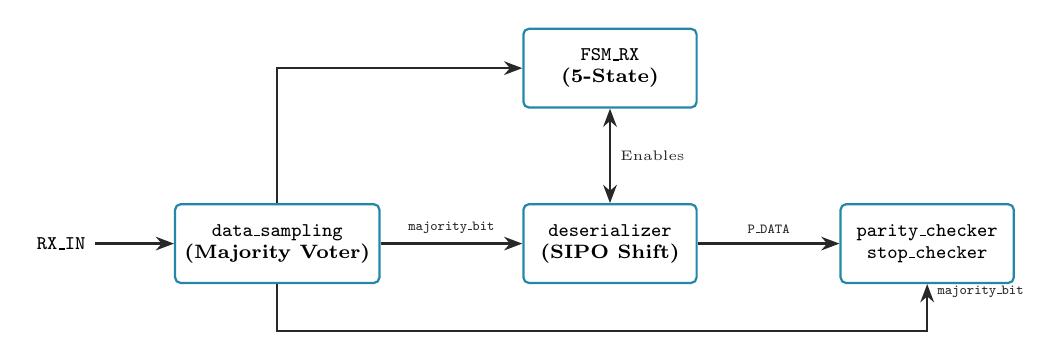
\begin{tikzpicture}[
    >=Stealth,
    node distance=1.8cm,
    block/.style={draw=primary, thick, fill=white, rounded corners=2pt, align=center, font=\scriptsize\bfseries, minimum height=1cm, minimum width=2.2cm},
    arrow/.style={->, thick, darkcharcoal}
]
    \node (rxin) [font=\scriptsize\bfseries] {\texttt{RX\_IN}};
    \node[block, right=1cm of rxin] (sampler) {\texttt{data\_sampling}\\(Majority Voter)};
    \node[block, right=of sampler] (deser) {\texttt{deserializer}\\(SIPO Shift)};
    \node[block, right=of deser] (checkers) {\texttt{parity\_checker}\\\texttt{stop\_checker}};
    \node[block, above=1.2cm of deser] (fsm) {\texttt{FSM\_RX}\\(5-State)};

    % Direct Path
    \draw[arrow] (rxin) -- (sampler);
    \draw[arrow] (sampler) -- node[above, font=\tiny] {\texttt{majority\_bit}} (deser);
    \draw[arrow] (deser) -- node[above, font=\tiny] {\texttt{P\_DATA}} (checkers);

    % Bypass Path (Routed cleanly underneath)
    \draw[arrow] (sampler.south) -- ++(0,-0.6) -| node[above right, near end, font=\tiny] {\texttt{majority\_bit}} (checkers.south);

    % FSM Path
    \draw[arrow] (sampler.north) |- (fsm.west);
    \draw[<->, thick, darkcharcoal] (fsm.south) -- node[right, font=\tiny] {Enables} (deser.north);

\end{tikzpicture}
\caption{UART Receiver Data Path and Error Checking Flow.}
\label{fig:uart_rx}
\end{figure}

\subsubsection{Architectural Function \& Mechanics}
The receiver captures incoming serial data on \texttt{RX\_IN} at $8\times$, $16\times$, or $32\times$ oversampling (Figure~\ref{fig:uart_rx}). It comprises seven modular sub-blocks:
\begin{itemize}
    \item \texttt{data\_sampling}: Samples the input stream at the center of the bit duration ($N/2-1$, $N/2$, $N/2+1$) and applies a \textbf{three-sample majority voting filter}:
    \begin{equation}
    \text{majority\_bit} = (S_1 \;\land\; S_2) \;\lor\; (S_1 \;\land\; S_3) \;\lor\; (S_2 \;\land\; S_3)
    \end{equation}
    \item \texttt{strt\_checker}: Evaluates the filtered start bit to reject false noise spikes.
    \item \texttt{deserializer}: Shifts 8 serial bits into a parallel byte register.
    \item \texttt{parity\_checker}: Checks parity checksum compliance and asserts \texttt{parity\_error}.
    \item \texttt{stop\_checker}: Verifies that the stop bit is logic 1 and asserts \texttt{framing\_error}.
    \item \texttt{edge\_bit\_counter}: Tracks intra-bit oversampling edges and inter-bit frame progress.
    \item \texttt{FSM\_RX}: 5-state receiver controller (\texttt{idle}, \texttt{start}, \texttt{data}, \texttt{parity}, \texttt{stop}).
\end{itemize}

\subsubsection{Design Rationale: Why 3-Sample Majority Voting Is Essential}
In real-world physical transmission environments, serial interconnects are subjected to electromagnetic interference (EMI), ground bounce, and clock frequency drift. A simple flip-flop sampler that takes a single snapshot at the clock edge is highly susceptible to corrupting entire data frames if a transient noise spike coincides with the sampling instant. The 3-sample majority voter samples the middle of the bit eye three consecutive times and takes the majority value, completely eliminating single-cycle noise glitches.

\subsubsection{Key Engineering Benefits}
\begin{itemize}
    \item \textbf{High Noise \& Spike Immunity}: Filters out line glitches shorter than half a bit period.
    \item \textbf{Real-Time Error Reporting}: Immediately alerts the system to transmission corruption via \texttt{parity\_error} and \texttt{framing\_error}.
    \item \textbf{Adaptive Oversampling}: Allows software to trade off receiver power consumption against noise margin ($8\times$ for low power, $32\times$ for maximum noise rejection).
\end{itemize}

% ------------------------------------------------------------------------------
% SECTION 6: DESIGN-SPACE EXPLORATION & TRADEOFF ANALYSIS
% ------------------------------------------------------------------------------
\section{Architectural Design-Space Exploration and Trade-Off Analysis}

To substantiate the microarchitectural choices made in this SoC, Table~\ref{tab:tradeoff_cdc} through Table~\ref{tab:tradeoff_pointers} provide rigorous comparative trade-off analyses against alternative design options.

\begin{table}[H]
\centering
\caption{Design-Space Exploration: Clock Domain Crossing (CDC) Strategies.}
\label{tab:tradeoff_cdc}
\footnotesize
\renewcommand{\arraystretch}{1.25}
\begin{tabularx}{\textwidth}{|>{\raggedright\arraybackslash}p{2.6cm}|c|c|c|Y|}
\hline
\textbf{CDC Technique} & \textbf{Latency} & \shortstack{\textbf{Bus}\\\textbf{Safety}} & \textbf{Throughput} & \shortstack{\textbf{Implementation}\\\textbf{Decision \& Rationale}} \\
\hline
\textbf{Direct Flip-Flop Array} & 2 cycles & \textcolor{cdcalert}{\textbf{FAIL}} & High & \textbf{Rejected}: Multi-bit skew causes catastrophic data incoherency. \\
\hline
\textbf{Asynchronous FIFO}      & 3--4 cycles & \textcolor{successgreen}{\textbf{PASS}} & Streaming & \textbf{Selected for Compute-to-UART Path}: Absorbs 100\,MHz burst data. \\
\hline
\textbf{Enable-Handshake Sync}   & 2--3 cycles & \textcolor{successgreen}{\textbf{PASS}} & Medium & \textbf{Selected for UART-to-FSM Path}: Coherent multi-bit transfer at minimal area. \\
\hline
\end{tabularx}
\end{table}

\begin{table}[H]
\centering
\caption{Design-Space Exploration: Clock Gating Architectures.}
\label{tab:tradeoff_cg}
\footnotesize
\renewcommand{\arraystretch}{1.25}
\begin{tabularx}{\textwidth}{|>{\raggedright\arraybackslash}p{2.6cm}|c|c|c|Y|}
\hline
\textbf{Gating Topology} & \shortstack{\textbf{Power}\\\textbf{Savings}} & \shortstack{\textbf{Glitch}\\\textbf{Risk}} & \shortstack{\textbf{Area \&}\\\textbf{Overhead}} & \shortstack{\textbf{Implementation}\\\textbf{Decision \& Rationale}} \\
\hline
\textbf{Software Multiplexing} & None & None & Moderate & \textbf{Rejected}: Clock tree continues toggling; zero dynamic power saved. \\
\hline
\textbf{Combinational AND Gate} & High & \textcolor{cdcalert}{\textbf{SEVERE}} & Minimal & \textbf{Rejected}: Generates fatal clock glitches on enable transitions. \\
\hline
\textbf{Latch-Based ICG Cell}  & Up to 80\% & \textcolor{successgreen}{\textbf{ZERO}} & Low & \textbf{Selected}: Eliminates glitches via active-low latch; maps to TSMC 130nm cell. \\
\hline
\end{tabularx}
\end{table}

\begin{table}[H]
\centering
\caption{Design-Space Exploration: Asynchronous Reset Distribution.}
\label{tab:tradeoff_reset}
\footnotesize
\renewcommand{\arraystretch}{1.25}
\begin{tabularx}{\textwidth}{|>{\raggedright\arraybackslash}p{2.6cm}|c|c|c|Y|}
\hline
\textbf{Reset Strategy} & \shortstack{\textbf{Power-On}\\\textbf{Safety}} & \shortstack{\textbf{Recovery}\\\textbf{Violations}} & \shortstack{\textbf{Skew}\\\textbf{Immunity}} & \shortstack{\textbf{Implementation}\\\textbf{Decision \& Rationale}} \\
\hline
\textbf{Pure Synchronous}  & Low & \textcolor{successgreen}{\textbf{None}} & Moderate & \textbf{Rejected}: Cannot initialize state if clock is dead at startup. \\
\hline
\textbf{Pure Asynchronous} & High & \textcolor{cdcalert}{\textbf{HIGH}} & Vulnerable & \textbf{Rejected}: Deassertion violates recovery time, desynchronizing FSMs. \\
\hline
\textbf{Async Assert / Sync Deassert} & High & \textcolor{successgreen}{\textbf{ZERO}} & Complete & \textbf{Selected}: Provides immediate reset with glitch-free synchronous release. \\
\hline
\end{tabularx}
\end{table}

\begin{table}[H]
\centering
\caption{Design-Space Exploration: FIFO Pointer Synchronization Encoding.}
\label{tab:tradeoff_pointers}
\footnotesize
\renewcommand{\arraystretch}{1.25}
\begin{tabularx}{\textwidth}{|>{\raggedright\arraybackslash}p{2.6cm}|c|c|c|Y|}
\hline
\textbf{Pointer Encoding} & \shortstack{\textbf{Toggles /}\\\textbf{Increment}} & \shortstack{\textbf{CDC}\\\textbf{Viability}} & \shortstack{\textbf{Area}\\\textbf{Overhead}} & \shortstack{\textbf{Implementation}\\\textbf{Decision \& Rationale}} \\
\hline
\textbf{Standard Binary}  & Up to $N$ bits & \textcolor{cdcalert}{\textbf{UNUSABLE}} & None & \textbf{Rejected}: Multi-bit transitions cause false full/empty triggers. \\
\hline
\textbf{One-Hot Encoding} & 2 bits & \textcolor{cdcalert}{\textbf{POOR}} & Exponential & \textbf{Rejected}: Area scales exponentially with depth ($2^N$ flops). \\
\hline
\textbf{Gray Code}        & Strictly 1 bit & \textcolor{successgreen}{\textbf{OPTIMAL}} & Low (XOR) & \textbf{Selected}: Single-bit change guarantees pointer coherency across CDC. \\
\hline
\end{tabularx}
\end{table}

% ------------------------------------------------------------------------------
% SECTION 7: VERIFICATION METHODOLOGY
% ------------------------------------------------------------------------------
\section{RTL Verification Methodology and Testbench Architecture}

\subsection{Automated Self-Checking Testbench}
Functional verification was executed using an automated, self-checking Verilog testbench~\cite{ieee_verilog} (\texttt{SYSTEM\_}\allowbreak\texttt{TOP\_}\allowbreak\texttt{tb.v}) developed for QuestaSim/ModelSim. The testbench features task-based serial stimulus drivers, expected-value checkers, and centralized error logging.

The test sequence executes the directed verification cases listed in Table~\ref{tab:testplan}. The protocol cases exercise the complete system path: host command bytes enter through \texttt{RX\_IN} and are decoded by the UART receiver and the master System Controller; the requested register content is then returned through the transmit path (including the asynchronous FIFO buffer) and validated on \texttt{TX\_OUT}. The testbench is organized around reusable Verilog \texttt{task} constructs that emulate the host-side physical interface:
\begin{itemize}
    \item \texttt{send\_bit} \& \texttt{send\_byte}: Drives the \texttt{RX\_IN} pin serially, calculating and injecting start, payload, programmable parity, and stop bits correctly synchronized to the \texttt{RX\_CLK} generated dynamically based on \texttt{REG2}.
    \item \texttt{write\_reg} \& \texttt{read\_reg\_and\_check}: Automates multi-byte register transactions using the host command opcodes \texttt{0xAA} (register write) and \texttt{0xBB} (register readback), including address transmission and readback validation.
    \item \texttt{check\_tx\_frame}: Implements robust timeout monitors (20,000 cycles) and sequentially validates the start bit, the eight payload bits (LSB-first), the expected dynamic parity bit when enabled, the stop bit, and the return of \texttt{TX\_OUT} to the idle level, without human visual inspection.
    \item \texttt{check\_value}: Performs immediate equivalence checking against golden expected bytes, logging failures dynamically.
\end{itemize}

\begin{table}[htbp]
\centering
\caption{Executed Verification Cases.}
\label{tab:testplan}
\small
\renewcommand{\arraystretch}{1.12}
\begin{tabularx}{\textwidth}{|c|l|c|Y|}
\hline
\textbf{Test ID} & \textbf{Verification Target} & \textbf{Status} & \textbf{Observed Verification Behavior} \\
\hline
\texttt{TC\_01} & Reset \& Default Check & \textcolor{successgreen}{\textbf{PASS}} & Reset released after 1,000\,ns; system settles for 100 \texttt{REF\_CLK} cycles before the first command. \\
\hline
\texttt{TC\_02} & Register File Write/Readback: Parity OFF (\texttt{0x55}) & \textcolor{successgreen}{\textbf{PASS}} & \texttt{0x55} written to \texttt{REG4} (parity off; \texttt{REG2}=\texttt{0x80}); direct register check and \texttt{0xBB} readback frame both matched. \\
\hline
\texttt{TC\_03} & Second Data Pattern (\texttt{0xA5}) & \textcolor{successgreen}{\textbf{PASS}} & \texttt{0xA5} written to \texttt{REG5}; register check and readback frame both matched. \\
\hline
\texttt{TC\_04} & Even Parity (\texttt{0x3C}) & \textcolor{successgreen}{\textbf{PASS}} & Even parity enabled (\texttt{REG2}=\texttt{0x81}); \texttt{0x3C} written to \texttt{REG6}; readback frame carried the correct even parity bit. \\
\hline
\texttt{TC\_05} & Odd Parity (\texttt{0x96}) & \textcolor{successgreen}{\textbf{PASS}} & Odd parity enabled (\texttt{REG2}=\texttt{0x83}); \texttt{0x96} written to \texttt{REG7}; readback frame carried the correct odd parity bit. \\
\hline
\texttt{TC\_06} & TX Frame-Format Validation & \textcolor{successgreen}{\textbf{PASS}} & Start bit, eight data bits (LSB-first), dynamic parity when enabled, stop bit, and idle return validated on every readback frame (20,000-cycle monitors). \\
\hline
\end{tabularx}
\end{table}

The archived regression run terminated with the success banner \texttt{ALL TESTS PASSED}; the transcript summary reports \texttt{Errors: 0, Warnings: 0}. The complete regression transcript and waveform log are archived with the project (transcript excerpt in Appendix~\ref{app:regression}). Additional scenarios---ALU command coverage, error injection, and FIFO stress---are identified as future verification extensions (see Section~\ref{sec:conclusion}).

% ------------------------------------------------------------------------------
% SECTION 8: SIMULATION RESULTS & WAVEFORM ANALYSIS
% ------------------------------------------------------------------------------
\section{Simulation Results and Waveform Analysis}

The complete self-checking regression testbench was executed in QuestaSim/ModelSim (Intel FPGA Edition v2020.1). All executed checks passed, including Parity Off (\texttt{0x55} injection), Second Data Pattern (\texttt{0xA5}), Even Parity (\texttt{0x3C}), and Odd Parity (\texttt{0x96}). Figures~\ref{fig:wave1}, \ref{fig:wave2}, and \ref{fig:wave3} present the recorded simulation waveforms across three key operational phases.

\begin{figure}[H]
\centering
\begin{tcolorbox}[colback=white, colframe=cardborder, boxrule=0.8pt, arc=2mm, left=4pt, right=4pt, top=4pt, bottom=4pt]
\waveformimage{modelsim_waveform_1.png}
\end{tcolorbox}
\caption{ModelSim Simulation Waveform 1: Clocks \& Resets (Gold/Red), Top-Level UART Serial I/O (Cyan/Green), UART RX/TX Subsystem, DATA\_SYNC CDC Handshake, and SYS\_CTRL Master FSM State Transitions across the complete test run.}
\label{fig:wave1}
\end{figure}

\vspace{0.4cm}

\begin{figure}[H]
\centering
\begin{tcolorbox}[colback=white, colframe=cardborder, boxrule=0.8pt, arc=2mm, left=4pt, right=4pt, top=4pt, bottom=4pt]
\waveformimage{modelsim_waveform_2.png}
\end{tcolorbox}
\caption{ModelSim Simulation Waveform 2: Master System Controller address/control generation, Register File write/readback transactions, and ALU 16-bit execution with gated clock activation.}
\label{fig:wave2}
\end{figure}

\vspace{0.4cm}

\begin{figure}[H]
\centering
\begin{tcolorbox}[colback=white, colframe=cardborder, boxrule=0.8pt, arc=2mm, left=4pt, right=4pt, top=4pt, bottom=4pt]
\waveformimage{modelsim_waveform_3.png}
\end{tcolorbox}
\caption{ModelSim Simulation Waveform 3: Asynchronous FIFO dual-clock buffering, write increment (\texttt{winc}), read increment (\texttt{rinc}), and full/empty flag status during burst transfers.}
\label{fig:wave3}
\end{figure}

% ------------------------------------------------------------------------------
% SECTION 9: SPYGLASS STATIC SIGN-OFF
% ------------------------------------------------------------------------------
\section{Synopsys SpyGlass Static Sign-off (Lint and CDC)}

Prior to logic synthesis, the RTL codebase was verified using Synopsys SpyGlass~\cite{spyglass} under the \path{GuideWare/latest/block/rtl_handoff} ruleset to ensure lint compliance and structural/functional CDC robustness.

\subsection{SpyGlass Lint Verification}
The lint run completed with \textbf{0 errors and 6 STARC05 warnings} (all waived after review): 2$\times$ \texttt{STARC05-1.4.3.4} --- divider output clock used as a non-clock signal (\texttt{Clk\_Div.v}); 4$\times$ \texttt{STARC05-2.11.3.1} --- combined combinational/sequential FSM coding style (\texttt{FIFO\_RD.v}, \texttt{FSM\_RX.v}, \texttt{Serializer.v}, \texttt{deserializer.v}). All were reviewed and waived, with no RTL changes required.
\begin{itemize}
    \item \textbf{No Unintended Latches}: Verified that all combinational always blocks provide complete case/if-else assignments, preventing inferred transparent latches.
    \item \textbf{Full Bus Width Compliance}: Verified that no implicit wire truncations, bit-width mismatches, or multi-driven nets exist.
    \item \textbf{FSM Reachability}: FSM encoding reviewed with default recovery to idle; no unreachable-state findings were reported by the lint ruleset.
\end{itemize}

\subsection{SpyGlass CDC Verification}
SpyGlass CDC validated the multi-clock domain crossings across both domains:
\begin{itemize}
    \item \textbf{Synchronization Topology Compliance}: Verified every asynchronous crossing is bound to an approved synchronization structure (two-flop metastability synchronizers, enable-handshake, Gray-coded FIFO pointers, quasi-static configuration paths); 0 unsynchronized crossings.
    \item \textbf{Gray-Code Pointer Verification}: Proved that the 4-bit write and read pointers in \texttt{ASYNC\_FIFO} strictly change by a Hamming distance of 1 per clock increment.
    \item \textbf{Convergence and Reconvergence Analysis}: One convergence point was identified --- the four synchronized Gray write-pointer bits converging on the read counter (\texttt{FIFO\_RD.rcounter[0]}); the Gray-encoding check PASSED, confirming a hazard-free converged path (structural-run warning waived after review).
    \item \textbf{Data-Enable Sequencing Advisories}: three transmit-path checks (\texttt{Ac\_datahold01a}; in \texttt{Parity\_Calc} and \texttt{Serializer}) were reported as partially proved with zero failing properties and were waived at sign-off.
\end{itemize}

% ------------------------------------------------------------------------------
% SECTION 10: SYNOPSYS DESIGN COMPILER LOGIC SYNTHESIS
% ------------------------------------------------------------------------------
\section{Synopsys Design Compiler Logic Synthesis}

Logic synthesis was conducted in \textbf{Synopsys Design Compiler}~\cite{synopsys_dc} targeting the \textbf{TSMC 130nm CMOS} standard-cell library (\texttt{scmetro\_tsmc\_cl013g\_rvt}).

\subsection{Synthesis Constraints and Corner Conditions}
The design was synthesized at the worst-case operational PVT corner condition:
\begin{itemize}
    \item \textbf{Process Corner}: Slow-Slow (SS) / 1.08\,V / 125$^\circ$C.
    \item \textbf{Reference Clock Constraint}: $f_{\text{REF\_CLK}} = 100.0\,\text{MHz}$ ($T_{\text{clk}} = 10.0\,\text{ns}$).
    \item \textbf{UART Clock Constraint}: $f_{\text{UART\_CLK}} = 3.6864\,\text{MHz}$ ($T_{\text{clk}} = 271.27\,\text{ns}$).
    \item \textbf{Clock Uncertainty}: Setup uncertainty = $0.2\,\text{ns}$, Hold uncertainty = $0.1\,\text{ns}$.
\end{itemize}

\subsection{Timing Closure and Area Results}
The synthesized gate-level netlist achieved complete zero-slack timing closure across all paths:
\begin{itemize}
    \item \textbf{Worst Negative Slack (Setup)}: \textbf{0.00\,ns} (MET across all 2,275 cells).
    \item \textbf{Worst Hold Slack}: \textbf{+0.43\,ns} (MET).
    \item \textbf{Critical Path}: Register File $\to$ ALU divider datapath $\to$ \texttt{ALU\_OUT[0]} register ($9.86\,\text{ns}$ data arrival).
\end{itemize}

A hierarchical breakdown of the synthesized standard-cell area is provided in Table~\ref{tab:area_breakdown}.

\begin{table}[H]
\centering
\caption{Synthesized Gate-Level Area Breakdown in TSMC 130nm CMOS (global cell area including sub-cells; source: \texttt{Synthesis/reports/area.rpt}).}
\label{tab:area_breakdown}
\small
\renewcommand{\arraystretch}{1.25}
\begin{tabularx}{\textwidth}{|Y|c|c|}
\hline
\textbf{Subsystem} & \textbf{Area ($\mu\text{m}^2$)} & \textbf{\% of Core} \\
\hline
\textbf{ALU (16-bit Engine)} & 8,864.08 & 32.6\% \\
\hline
\textbf{RegFile ($16\times 8$-bit)} & 6,045.88 & 22.2\% \\
\hline
\textbf{ASYNC\_FIFO (Dual-Clock)} & 4,103.15 & 15.1\% \\
\hline
\textbf{UART Subsystem (TX + RX)} & 3,730.14 & 13.7\% \\
\hline
\textbf{U0\_TX\_CLK\_DIV} & 1,269.66 & 4.7\% \\
\hline
\textbf{U1\_RX\_CLK\_DIV} & 1,269.66 & 4.7\% \\
\hline
\textbf{SYS\_CTRL (Master FSM)} & 1,203.76 & 4.4\% \\
\hline
\textbf{Syncs, Pulse\_Gen, Mux, CLK\_GATE, top glue} & 738.97 & 2.7\% \\
\hline
\textbf{Total Core} & \textbf{27,225.31} & \textbf{100.0\%} \\
\hline
\end{tabularx}
\end{table}

% ------------------------------------------------------------------------------
% SECTION 11: SYNOPSYS DFT COMPILER
% ------------------------------------------------------------------------------
\section{Synopsys DFT Compiler (Design-for-Testability)}

Manufacturing testability was integrated via \textbf{Synopsys DFT Compiler}~\cite{synopsys_dft} using standard full-scan insertion methodology:
\begin{itemize}
    \item \textbf{Scan Cell Replacement}: All 380 scan flip-flops were replaced with multiplexed-D scan flip-flops (\texttt{SDFF}) from the TSMC 130nm library; the design's 380 scan cells are grouped into four fully balanced chains of 95 cells each.
    \item \textbf{Scan Chain Architecture}: Four balanced scan chains, 95 cells each (\texttt{SI[3:0]} $\to$ \texttt{SO[3:0]}), were inserted to maximize ATPG pattern shift parallelism and reduce automatic test equipment (ATE) test time.
    \item \textbf{Clock Domain Isolation}: Scan chains were partitioned such that flip-flops belonging to \texttt{REF\_CLK} and \texttt{UART\_CLK} are isolated during shift mode, preventing scan-shift clock skew race hazards.
\end{itemize}

The resulting testability sign-off metrics are summarized in Table~\ref{tab:dft_metrics}.

\begin{table}[H]
\centering
\caption{Synopsys DFT Compiler Testability Sign-off Metrics.}
\label{tab:dft_metrics}
\renewcommand{\arraystretch}{1.3}
\begin{tabularx}{\textwidth}{|l|c|Y|}
\hline
\textbf{Testability Parameter} & \textbf{Achieved Value} & \textbf{Sign-off Verification Description} \\
\hline
\textbf{Total Scan Flip-Flops} & 380 Flops & 4 balanced chains $\times$ 95 cells. \\
\hline
\textbf{Scan Chain Lengths} & 95 / 95 / 95 / 95 & Fully balanced (logged by DFT Compiler). \\
\hline
\textbf{Test Coverage} & \textbf{99.66\%} & Estimate over 17,638 collapsed faults. \\
\hline
\textbf{Fault Classes} & 17,305 DT / 1 PT / 273 UD / 48 AU / 11 ND & Detected / possibly detected / undetectable / ATPG-untestable / not detected. \\
\hline
\end{tabularx}
\end{table}

% ------------------------------------------------------------------------------
% ------------------------------------------------------------------------------
% SECTION 12: PHYSICAL DESIGN IMPLEMENTATION (PLACE AND ROUTE & SIGN-OFF)
% ------------------------------------------------------------------------------
% [W6 PnR region --- new section spliced between Section 11 (DFT) and Section 13 (Formality).
%  Defines labels: sec:pnr, tab:pnr_params, tab:pnr_signoff, tab:pnr_exports, fig:asic_flow, fig:layout_floorplan, fig:layout_physical.
%  Figure dependency: figures/floorplan_view.png, figures/physical_view.png. The fig:asic_flow tikz below extends the original flow figure.]
\section{Physical Design Implementation: Place and Route and Sign-off}
\label{sec:pnr}

\subsection{Flow Overview and Setup}
The physical implementation of \texttt{SYS\_TOP} was carried out in Cadence First Encounter v08.10-p004 with the embedded NanoRoute v08.10-p008 router~\cite{cadence_encounter}, starting from the post-DFT gate-level netlist (\texttt{DFT/netlists/SYS\_TOP.v}) and its timing constraints (\texttt{SYS\_TOP.sdc}). A multi-mode multi-corner (MMMC) configuration drove all analysis: three constraint modes (functional, scan, and capture) were combined with the minimum and maximum cell libraries (\texttt{ff\_1p32v\_m40c} / \texttt{ss\_1p08v\_125c}; a typical library \texttt{tt\_1p2v\_25c} was also loaded), producing six analysis views (setup and hold views for each mode) over a single extracted RC corner.

The complete session was executed on October 4, 2026 and ran for approximately 19 minutes (23:37--23:55), carrying the design from floorplanning through routing, sign-off, and GDSII export with no unresolved violations. The executed command sequence is archived with the flow scripts (Appendix~\ref{app:flow}). Figure~\ref{fig:asic_flow} shows the extended RTL-to-GDSII flow, and Table~\ref{tab:pnr_params} summarizes the place-and-route setup.

\begin{figure}[H]
\centering
\resizebox{\linewidth}{!}{%
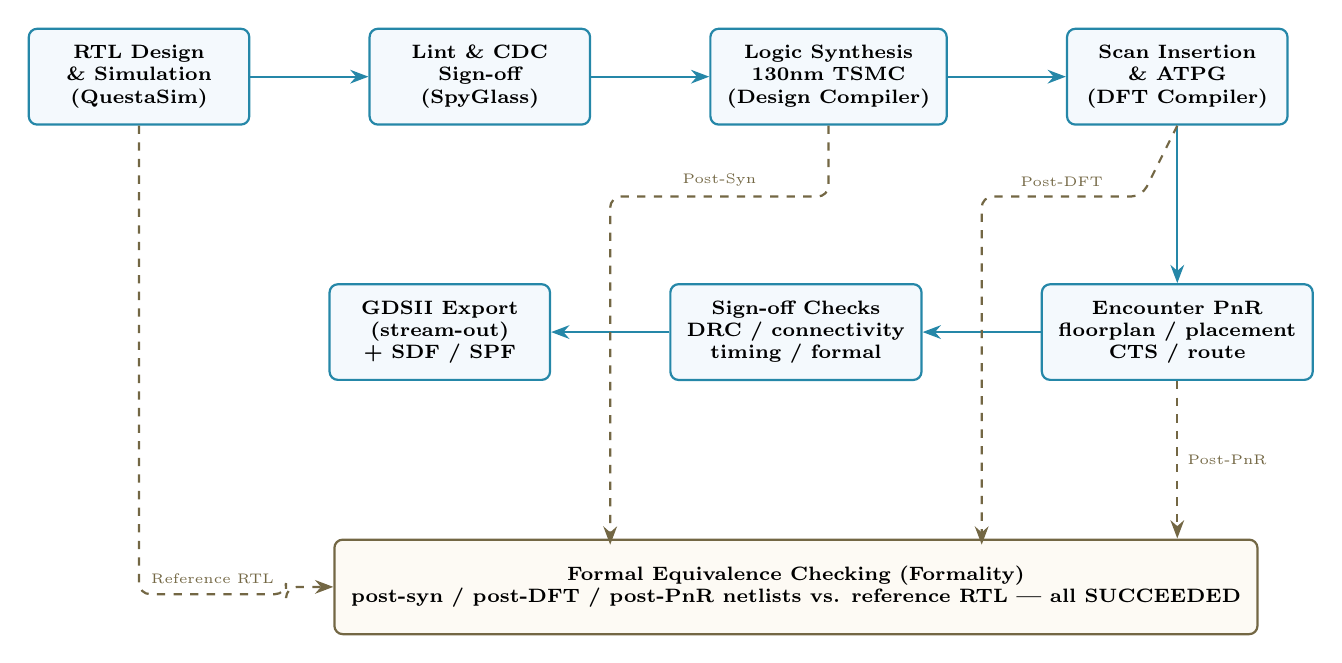
\begin{tikzpicture}[
    >=Stealth,
    node distance=1.5cm,
    toolbox/.style={draw=primary, thick, fill=uartbg, rounded corners=3pt, align=center, font=\scriptsize\bfseries, inner sep=6pt, minimum width=2.8cm, minimum height=1.2cm},
    arrow/.style={->, thick, primary},
    dashed_arrow/.style={->, dashed, thick, accent}
]
    % Main RTL-to-GDSII flow
    \node[toolbox] (rtl) {RTL Design\\\& Simulation\\(QuestaSim)};
    \node[toolbox, right=of rtl] (spyglass) {Lint \& CDC\\Sign-off\\(SpyGlass)};
    \node[toolbox, right=of spyglass] (dc) {Logic Synthesis\\130nm TSMC\\(Design Compiler)};
    \node[toolbox, right=of dc] (dft) {Scan Insertion\\\& ATPG\\(DFT Compiler)};
    \node[toolbox, below=2cm of dft] (pnr) {Encounter PnR\\floorplan / placement\\CTS / route};
    \node[toolbox, left=of pnr] (signoff) {Sign-off Checks\\DRC / connectivity\\timing / formal};
    \node[toolbox, left=of signoff] (gdsii) {GDSII Export\\(stream-out)\\+ SDF / SPF};

    % Formal equivalence checking node
    \node[toolbox, fill=refbg, draw=accent, minimum width=11.5cm, below=2cm of signoff] (formality) {Formal Equivalence Checking (Formality)\\{post-syn / post-DFT / post-PnR netlists vs. reference RTL --- all SUCCEEDED}};

    % Chain arrows
    \draw[arrow] (rtl) -- (spyglass);
    \draw[arrow] (spyglass) -- (dc);
    \draw[arrow] (dc) -- (dft);
    \draw[arrow] (dft) -- (pnr);
    \draw[arrow] (pnr) -- (signoff);
    \draw[arrow] (signoff) -- (gdsii);

    % Formality tap points
    \coordinate (psmid) at ($(gdsii.east)!.5!(signoff.west)$);
    \coordinate (pdmid) at ($(signoff.east)!.5!(pnr.west)$);
    \coordinate (fmA) at ($(psmid) + (0,-2.7)$);
    \coordinate (fmB) at ($(pdmid) + (0,-2.7)$);
    \coordinate (fmC) at ($(pnr.south) + (0,-2.0)$);

    % Formal equivalence check arrows
    \draw[dashed_arrow, rounded corners] (rtl.south) -- ++(0,-5.95) -| node[above, near start, font=\tiny, text=accent] {Reference RTL} ($(formality.west)+(-0.6,0)$) -- (formality.west);
    \draw[dashed_arrow, rounded corners] (dc.south) -- ++(0,-0.9) -| node[above, near start, font=\tiny, text=accent] {Post-Syn} (fmA);
    \draw[dashed_arrow, rounded corners] (dft.south) -- ++(-0.45,-0.9) -| node[above, near start, font=\tiny, text=accent] {Post-DFT} (fmB);
    \draw[dashed_arrow] (pnr.south) -- node[right, font=\tiny, text=accent] {Post-PnR} (fmC);

\end{tikzpicture}
}
\caption{Complete RTL-to-GDSII implementation and sign-off flow (Cadence Encounter 8.10 with NanoRoute; physical sign-off checks; formal equivalence across the post-synthesis, post-DFT, and post-route netlists).}
\label{fig:asic_flow}
\end{figure}

\begin{table}[H]
\centering
\caption{Cadence Encounter Physical Implementation Flow Parameters.}
\label{tab:pnr_params}
\small
\renewcommand{\arraystretch}{1.25}
\begin{tabularx}{\textwidth}{|l|Y|l|}
\hline
\textbf{Parameter} & \textbf{Value} & \textbf{Source} \\
\hline
Tool / version & Cadence First Encounter v08.10-p004 with embedded NanoRoute v08.10-p008 & \texttt{encounter.log} \\
\hline
Technology & 0.13\,$\mu$m CMOS, 7-metal FSG stack (\texttt{tsmc13fsg\_7lm\_tech.lef}); Metro \texttt{cl013g} RVT cells & \texttt{des\_import.tcl} \\
\hline
Timing corners & min \texttt{ff\_1p32v\_m40c}, max \texttt{ss\_1p08v\_125c}, typical \texttt{tt\_1p2v\_25c}; single extracted RC corner & \texttt{MMMC.tcl} \\
\hline
Analysis views & 3 constraint modes (functional / scan / capture) $\times$ 2 corners = 6 views (setup 1--3, hold 1--3) & \texttt{MMMC.tcl} \\
\hline
Die and core & die 240.47\,$\times$\,220.47\,$\mu$m with 6\,$\mu$m margins; core box 228.32\,$\times$\,208.32\,$\mu$m & \texttt{SYS\_TOP.fp} \\
\hline
I/O pins & 19 ports (11 single-bit + \texttt{SI[3:0]} + \texttt{SO[3:0]}) & \texttt{encounter.log} \\
\hline
Row architecture & site \texttt{TSM130NMMETROSITE}, 556 sites per row, 2.87\,$\mu$m row pitch & \texttt{SYS\_TOP.fp} \\
\hline
PG ring & width 2\,$\mu$m, spacing 0.5\,$\mu$m; METAL5 top/bottom + METAL6 left/right; stacked vias METAL1 to METAL7 & \texttt{encounter.log} \\
\hline
PG stripes & METAL6, width 1\,$\mu$m, pitch 60\,$\mu$m, spacing 0.5\,$\mu$m & \texttt{encounter.log} \\
\hline
Placement & \texttt{placeDesign -inPlaceOpt -prePlaceOpt}; density 56.8\% (26,751\,$\mu$m$^2$ cell area) & \texttt{encounter.log} \\
\hline
CTS & \texttt{clockDesign -specFile Clock.ctstch -fixedInstBeforeCTS}; skew target 200\,ps, transition target 50\,ps & \texttt{Clock.ctstch} \\
\hline
Routing & \texttt{routeDesign -globalDetail -viaOpt -wireOpt}; 6 metal layers used (M1--M6) & \texttt{routing.tcl} \\
\hline
Fill & seven \texttt{FILL} sizes (\texttt{FILL1M}--\texttt{FILL64M}), 3,145 filler cells, FIXED mode & \texttt{encounter.log} \\
\hline
Reference clocks & \texttt{REF\_CLK} 10\,ns (100\,MHz); \texttt{UART\_CLK} 271.267\,ns; scan clock \texttt{dft\_clk} 1000\,ns & \texttt{SYS\_TOP.sdc} \\
\hline
Constraints & setup uncertainty 0.2\,ns / hold 0.1\,ns; clock transition 0.05\,ns; scan I/O delay 200\,ns; \texttt{test\_mode} = 1, \texttt{SE} = 0 case analysis & \texttt{SYS\_TOP.sdc} \\
\hline
\end{tabularx}
\end{table}

\subsection{Floorplanning and Power Planning}
\begin{sloppypar}
The die was sized with \texttt{floorPlan -d 240.47 220.47 6.0 6.0 6.0 6.0}, producing a 240.47\,$\times$\,220.47\,$\mu$m die with nominal 6\,$\mu$m margins on all sides and a core box of 228.32\,$\times$\,208.32\,$\mu$m. Standard-cell rows use the \texttt{TSM130NMMETROSITE} site with 556 sites per row at a 2.87\,$\mu$m row pitch.
\end{sloppypar}

The power distribution network consists of a supply ring 2\,$\mu$m wide (METAL5 along the top and bottom edges, METAL6 along the left and right edges, stitched with stacked vias from METAL1 to METAL7) and METAL6 stripes 1\,$\mu$m wide at a 60\,$\mu$m pitch. Special routing (\texttt{sroute}) then connected the supply network, routing 146 core power ports and 73 follow-pin connections; only the warnings expected of a pre-placement power route were reported, and supply integrity was later confirmed clean by the post-route connectivity check discussed below. Figure~\ref{fig:layout_floorplan} shows the resulting floorplan with the completed power distribution network.

\begin{figure}[H]
\centering
\begin{tcolorbox}[colback=white, colframe=cardborder, boxrule=0.8pt, arc=2mm, left=4pt, right=4pt, top=4pt, bottom=4pt]
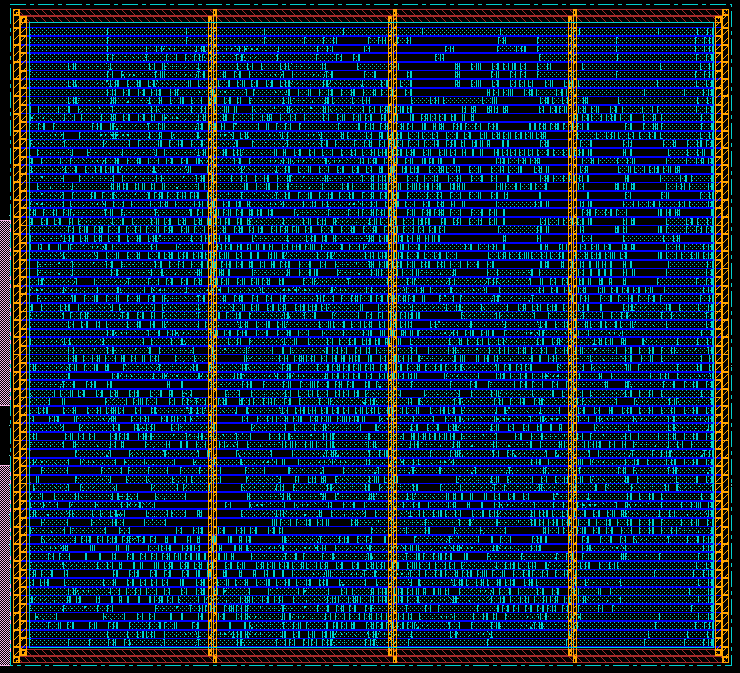
\includegraphics[width=\linewidth]{floorplan_view.png}
\end{tcolorbox}
\caption{SYS\_TOP floorplan with the power distribution network --- floorplan view captured from the Encounter database (die 240.47\,$\times$\,220.47\,$\mu$m; power ring and METAL6 straps over the standard-cell rows).}
\label{fig:layout_floorplan}
\end{figure}

\subsection{Placement}
Standard cells were placed with timing-driven optimization (\texttt{placeDesign -inPlaceOpt -prePlaceOpt}). The placed design reached a density of 56.8\% (26,751\,$\mu$m$^2$ of standard-cell area) with zero unplaced instances; detailed placement refined 885 instances. Seven tie-off cells (3\,$\times$ \texttt{TIELOM}, 4\,$\times$ \texttt{TIEHIM}) were inserted to tie unused inputs and connected to the power and ground network. The pre-CTS timing check reported a setup worst negative slack (WNS) of +4.315\,ns with zero violating paths across all six analysis views.

\subsection{Clock Tree Synthesis}
Clock tree synthesis (CTS) was specified with a maximum skew target of 200\,ps and a sink transition target of 50\,ps, and was built with \texttt{clockDesign -specFile Clock.ctstch -fixedInstBeforeCTS} for the three clock trees: the scan clock \texttt{dft\_clk} (reported as \texttt{scan\_clk}), \texttt{UART\_CLK}, and \texttt{REF\_CLK}. Because \texttt{-fixedInstBeforeCTS} was used, the clock cells were excluded from subsequent placement changes. The final routed clock trees achieved:
\begin{itemize}
    \item scan clock: 64 buffers, 376 sinks, 20 levels, worst skew 159\,ps (hold 94.3\,ps) against the 200\,ps requirement;
    \item \texttt{UART\_CLK}: 29 buffers, 110 sinks, 17 levels, 124.7\,ps (hold 52.4\,ps);
    \item \texttt{REF\_CLK}: 19 buffers, 249 sinks, 9 levels, 13.5\,ps (hold 11.6\,ps).
\end{itemize}
The initial post-CTS hold check exposed a worst hold slack of $-0.724$\,ns across 328 violating paths (total negative slack $-88.533$\,ns), which was fixed with \texttt{optDesign -postCTS -hold}: 19 cells were added (14\,$\times$ \texttt{DLY4X1M}, 1\,$\times$ \texttt{DLY2X1M}, 2\,$\times$ \texttt{DLY1X1M}, 2\,$\times$ \texttt{BUFX2M}) to restore positive hold slack (+0.014\,ns) without disturbing the setup result.

\subsection{Routing and Chip Finish}
Routing was executed with NanoRoute using global and detailed routing together with via and wire optimization (\texttt{routeDesign -globalDetail -viaOpt -wireOpt}); 84 clock nets (3.62\%) were given an additional preferred spacing class to protect the clock network. The final routed design contains 70,072\,$\mu$m of wire length, dominated by METAL2 (29.68\,mm) and METAL3 (26.31\,mm), and 16,708 vias of which 32.6\% are multi-cut; the route completed with 0 DRC violations and 0 route failures after optimization resolved the initial markers.

Chip finish added 3,145 filler cells across seven \texttt{FILL} sizes in FIXED mode to complete the rows; the filler self-check reported 0 DRC violations and \texttt{checkFiller} found 0 gaps, finalizing the row-based layout. Figure~\ref{fig:layout_physical} shows the final routed layout as displayed in the Encounter physical view.

\begin{figure}[H]
\centering
\begin{tcolorbox}[colback=white, colframe=cardborder, boxrule=0.8pt, arc=2mm, left=4pt, right=4pt, top=4pt, bottom=4pt]
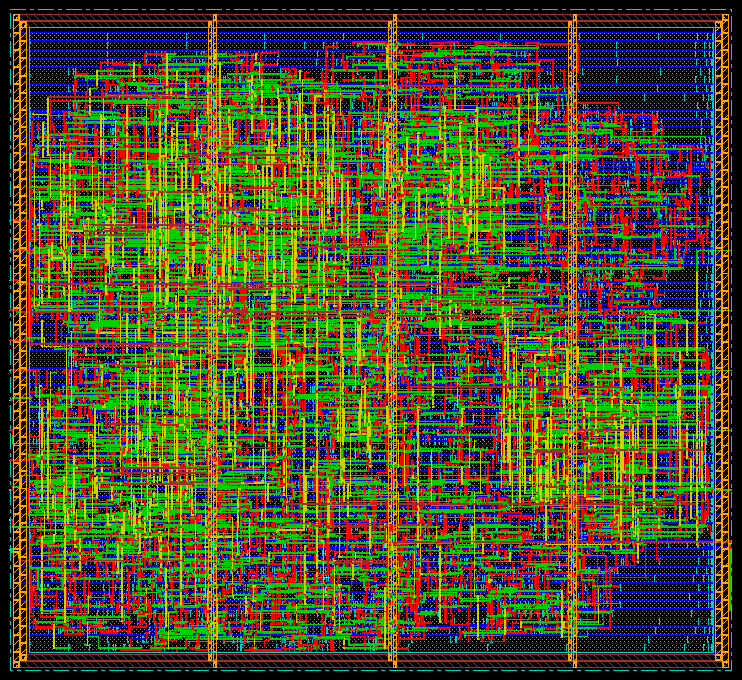
\includegraphics[width=\linewidth]{physical_view.png}
\end{tcolorbox}
\caption{SYS\_TOP final routed layout --- physical view captured from the Encounter database (standard-cell rows with clock tree and multi-layer signal routing; die 240.47\,$\times$\,220.47\,$\mu$m).}
\label{fig:layout_physical}
\end{figure}

\subsection{Physical Verification and Sign-off}
With routing and chip finish complete, the final database was checked with Encounter's built-in verifiers and static timing analysis. The sign-off results are collected in Table~\ref{tab:pnr_signoff} and summarized below:
\begin{itemize}
    \item \textbf{Geometry (DRC)}: \texttt{verifyGeometry -noMinArea} reported zero violations in every category (cells, same-net, wiring, antenna, shorts, and overlaps); the check was run both before and after filler insertion.
    \item \textbf{Connectivity}: \texttt{verifyConnectivity -type all} reported no problems or warnings across the routed design.
    \item \textbf{Process antenna}: \texttt{verifyProcessAntenna} reported 0 violations.
    \item \textbf{Static timing (post-route)}: setup WNS +4.409\,ns (TNS 0.000\,ns, 0 violating paths of 1,144) and hold WNS +0.015\,ns (TNS 0.000\,ns, 0 violating), across all six analysis views.
    \item \textbf{Design rule violations}: maximum capacitance, maximum transition, and maximum fanout checks all report zero violations.
    \item \textbf{Power estimate}: 1.212\,mW total at the \texttt{ss\_1p08v\_125c} corner with \texttt{VDD} = 1.08\,V and primary input activity 0.2; the estimate is vectorless and includes scan-clock activity (\texttt{dft\_clk} contributes 48.39\% of the total).
    \item \textbf{Formal equivalence}: the formal equivalence of the post-route netlist is covered in Section~\ref{sec:formality}; in summary, verification SUCCEEDED with 361 passing compare points and 0 failing.
\end{itemize}

\begin{table}[htbp]
\centering
\caption{Post-Route Sign-off Results for \texttt{SYS\_TOP}.}
\label{tab:pnr_signoff}
\small
\renewcommand{\arraystretch}{1.25}
\begin{tabularx}{\textwidth}{|>{\raggedright\arraybackslash}p{3.4cm}|>{\raggedright\arraybackslash}p{4.6cm}|Y|}
\hline
\textbf{Metric} & \textbf{Result} & \textbf{Condition / Note} \\
\hline
Setup timing & +4.409\,ns / 0.000\,ns / 0 & WNS / TNS / violating paths; 1,144 paths across all six views \\
\hline
Hold timing & +0.015\,ns / 0.000\,ns / 0 & WNS / TNS / violating paths; post-filler re-run \\
\hline
Design rule violations & max\_cap 0, max\_tran 0, max\_fanout 0 & real and total counts, post-route \\
\hline
Clock skew (routed) & 159 / 124.7 / 13.5\,ps (setup); 94.3 / 52.4 / 11.6\,ps (hold) & scan / \texttt{UART\_CLK} / \texttt{REF\_CLK}; requirement 200\,ps \\
\hline
Routed wirelength & 70,072\,$\mu$m total & dominated by METAL2 (29.68\,mm) and METAL3 (26.31\,mm) \\
\hline
Vias & 16,708 total; 32.6\% multi-cut & single-cut 11,261; via and wire optimization applied \\
\hline
Density & 60.30\% before fill; 100.000\% after fill & placement check vs. post-filler reporting \\
\hline
Geometry (DRC) & 0 violations (all classes) & \texttt{verifyGeometry -noMinArea}; run pre- and post-filler \\
\hline
Connectivity & no problems or warnings & \texttt{verifyConnectivity -type all} \\
\hline
Antenna & 0 violations & \texttt{verifyProcessAntenna} \\
\hline
Power (post-route estimate) & 1.212\,mW total & \texttt{ss\_1p08v\_125c}, \texttt{VDD} = 1.08\,V, input activity 0.2; vectorless; includes scan-clock activity (\texttt{dft\_clk} 48.39\%) \\
\hline
Cells / nets & 2,160 leaf cells + 3,145 fillers; 2,276 nets & fillers are physical-only; 5,305 instances in GDSII \\
\hline
Formal equivalence & SUCCEEDED --- 361 / 361 passing, 0 failing & reference RTL vs. post-route netlist; details in Section~\ref{sec:formality} \\
\hline
\end{tabularx}
\end{table}

\subsection{GDSII Export and Deliverables}
The signed-off database was exported for hand-off: GDSII via \texttt{streamOut} (units 2000 DBU, all layers), a version-3.0 SDF back-annotation file via \texttt{delayCal -sdf}, extracted parasitics via \texttt{rcOut -spf}, gate-level netlists via \texttt{saveNetlist} (both plain and with power/ground connections), and the saved Encounter database (\texttt{SYS\_TOP\_Final\_Chip.enc}). The exported files are listed in Table~\ref{tab:pnr_exports}.

\begin{table}[htbp]
\centering
\caption{Exported Implementation Deliverables and File Sizes.}
\label{tab:pnr_exports}
\renewcommand{\arraystretch}{1.2}
\begin{tabularx}{\textwidth}{|l|Y|l|}
\hline
\textbf{File} & \textbf{Contents} & \textbf{Size} \\
\hline
\texttt{SYS\_TOP.gds} & GDSII stream-out (2000 DBU, full design) & 260,978 B \\
\hline
\texttt{SYS\_TOP.sdf} & SDF version 3.0 timing back-annotation & 2.99 MB \\
\hline
\texttt{SYS\_TOP.spf} & Extracted parasitic model (\texttt{rcOut -spf}) & 6.61 MB \\
\hline
\texttt{SYS\_TOP.v} & Post-route gate-level netlist & 250,239 B \\
\hline
\texttt{SYS\_TOP\_pg.v} & Netlist with power/ground connections & 306,635 B \\
\hline
\end{tabularx}
\end{table}

The SDF (version 3.0) and the SPF export are provided for downstream static timing and parasitic analysis of the routed netlist. The stream-out completed successfully; layer-mapping diagnostics emitted during export are retained as a follow-up item for downstream reference-deck checking. The layout views captured from the saved Encounter database are presented earlier in this section (Figures~\ref{fig:layout_floorplan} and~\ref{fig:layout_physical}).

% (rendered placement-map figure removed --- replaced by captured floorplan/physical views above)

% ---- Gate-Level Simulation (Post-Route SDF) ----
\subsection{Gate-Level Simulation (Post-Route SDF)}
\label{subsec:gls}

As a final functional check on the implemented netlist, the exported post-route gate-level netlist and its version-3.0 SDF file (Table~\ref{tab:pnr_exports}) were re-simulated with the same self-checking regression testbench used at the RTL stage (Table~\ref{tab:testplan}), compiled against the TSMC 130\,nm standard-cell simulation models. The run was executed in QuestaSim~10.7c with the SDF applied in \texttt{-sdfmax} mode, i.e.\ at the maximum (slow) delays corresponding to 1.08\,V and 125\,$^\circ$C as recorded in the SDF header --- the setup-critical condition for timing sign-off.

SDF back-annotation completed successfully and the full directed regression ran to completion: all checks passed, terminating with the \texttt{ALL TESTS PASSED} banner and the simulator's \texttt{[SIMULATION SUCCESSFUL]} status after $\approx 3.2$\,ms of simulated system operation ($\approx 17$\,s of wall-clock simulation time). The simulator's timing checks flagged three setup-time events, all on the first stage of the \texttt{DATA\_SYNC} synchronizer (\texttt{multi\_flops\_reg[0]}); these are the expected consequence of sampling the asynchronous \texttt{bus\_enable} input close to a clock edge and are resolved by the two-stage synchronizer by design --- no functional check failed. The remaining console output consists of SDF-to-model mapping notices (missing \texttt{specify} coverage in the cell simulation models, and post-PnR instance/port name mapping), which are tool-flow messages rather than design issues.

The gate-level pass completes the verification stack for the delivered netlist: it is formally equivalent to the RTL (Section~\ref{sec:formality}), meets the post-route static timing sign-off (Table~\ref{tab:pnr_signoff}), and reproduces the complete directed regression functionally correct under real back-annotated delays. The full-hierarchy switching-activity trace (VCD) captured during this run is reused as the activity source for the VCD-annotated power analysis of Section~\ref{subsec:px}.
% SECTION 13: SYNOPSYS FORMALITY FORMAL EQUIVALENCE
% ------------------------------------------------------------------------------
\section{Synopsys Formality Formal Equivalence Verification}
\label{sec:formality}

Formal Equivalence Checking (LEC) was executed using \textbf{Synopsys Formality}~\cite{synopsys_fm} across three sign-off stages (post-synthesis, post-DFT, and post-place-and-route). Figure~\ref{fig:asic_flow} (Section~\ref{sec:pnr}) illustrates the verification phases within the complete backend flow. The physical implementation itself is described in Section~\ref{sec:pnr}.

All three formal runs converged with \textbf{100\% Comparison Success}:
\begin{itemize}
    \item \textbf{Post-Synthesis} (RTL vs.\ post-synthesis netlist): \textbf{379} compare points (375 DFF + 3 ports + 1 latch); verification \textbf{SUCCEEDED}.
    \item \textbf{Post-DFT} (pre-DFT vs.\ post-DFT netlist; scan chain insertion, mission mode): \textbf{361} compare points (358 DFF + 3 ports); verification \textbf{SUCCEEDED}.
    \item \textbf{Post-PnR} (post-DFT vs.\ post-PnR netlist; SI/SO scan ports excluded): \textbf{361} compare points (358 DFF + 3 ports); verification \textbf{SUCCEEDED}.
\end{itemize}

In total, \textbf{0} failing and \textbf{0} unmatched compare points; two reference registers (deserializer \texttt{counter\_reg[3]}, \texttt{data\_reg[7]}) were reported as unread (optimized in the implementation netlist) and excluded via standard unread/constant handling.

% ------------------------------------------------------------------------------
% SECTION 14: POWER ANALYSIS & OPTIMIZATION
% ------------------------------------------------------------------------------
\section{Power Optimization and Dynamic Power Profiling}
\label{sec:power}

The ALU datapath is idle during most UART-dominated execution cycles, so its clock branch is gated by a latch-based Integrated Clock Gating (ICG) cell. The \texttt{CLK\_GATE} module instantiates the TSMC 130nm library ICG cell (\texttt{TLATNCAX2M}) in synthesis mode; its enable (\texttt{Gate\_EN}) is asserted by the master FSM only during ALU execution, and the active-low latch captures the enable in the clock-low phase, keeping the gated clock glitch-free.

Power was profiled in the Synopsys DC/Power Compiler flow at 100\,MHz; the conditions for each estimate are noted below.
\begin{itemize}
    \item \textbf{Synthesis estimate} (\texttt{Synthesis/reports/power.rpt}; SS/1.08\,V/125\,$^\circ$C corner; default propagated activity --- primary inputs unannotated, low-effort vectorless simulation): total $\approx 0.484\,\text{mW}$ (internal $0.412\,\text{mW}$, switching $54.7\,\mu\text{W}$, leakage $18.2\,\mu\text{W}$).
    \item \textbf{Post-scan estimate} (\texttt{DFT/reports/power.rpt}): total $\approx 0.166\,\text{mW}$ (leakage $15.6\,\mu\text{W}$).
    \item \textbf{Post-route estimate} (\texttt{System\_pnr/pnr/report/power.rpt}; primary-input activity 0.2): total $1.212\,\text{mW}$ at $1.08\,\text{V}$ (internal 70.3\%, switching 28.1\%, leakage 1.6\% $\approx 19.9\,\mu\text{W}$). This figure includes the DFT scan-clock domain ($\approx 48\%$ of the total power) and therefore overestimates functional-mode power; the VCD-annotated analysis below quantifies the functional-mode figure.
\end{itemize}

All estimates above use default or vectorless activity where noted. To complement them, a switching-activity-annotated analysis was performed on the post-route netlist using the activity trace captured during the gate-level regression, as described next.

% ---- VCD-Annotated Power Analysis (PrimeTime PX) ----
\subsection{VCD-Annotated Power Analysis (PrimeTime PX)}
\label{subsec:px}

A time-based power analysis was executed with Synopsys PrimeTime PX (O-2018.06-SP1) on the post-route netlist, driven by the VCD switching-activity trace captured during the gate-level regression of Section~\ref{subsec:gls}. Because the activity is taken from the actual functional run --- including the real clock-gating behavior of the ALU and the genuine \texttt{REF\_CLK}/\texttt{UART\_CLK} activity over $\approx 3.2$\,ms --- the result characterizes normal operation rather than assumed activity factors. The session resolves the typical-corner library (TT: 1.2\,V, 25\,$^\circ$C).

\begin{table}[htbp]
\centering
\caption{PrimeTime PX VCD-annotated power summary for the post-route netlist (functional workload).}
\label{tab:px_power}
\renewcommand{\arraystretch}{1.2}
\begin{tabularx}{\textwidth}{|Y|c|c|}
\hline
\textbf{Power Component} & \textbf{Value} & \textbf{Share of Total} \\
\hline
Net switching power & $0.67\,\mu$W & 5.7\% \\
\hline
Cell internal power & $3.21\,\mu$W & 27.4\% \\
\hline
Cell leakage power & $7.84\,\mu$W & 66.9\% \\
\hline
\textbf{Total power} & \textbf{11.72\,$\mu$W} & 100\% \\
\hline
\end{tabularx}
\end{table}

Two run conditions are noted for completeness: clock definitions were not applied in this first analysis session (clock-network and register power are therefore not separately attributed), and PrimeTime reports partial VCD coverage with its power-may-be-underestimated warning; the reported total is consequently treated as a \emph{lower bound} for functional-mode power, with a clock- and SDF-loaded rerun at fuller coverage identified as a refinement step. Even as a lower bound, the result quantitatively confirms the low-power behavior of the design under normal operation: with the scan clock idle and a UART-dominated workload, the reported average power is leakage-dominated ($\approx 67\%$) and lies roughly two orders of magnitude below the scan-inclusive, slow-corner post-route estimate of the item above.

% ------------------------------------------------------------------------------
% SECTION 15: SUMMARY OF IMPLEMENTATION RESULTS
% ------------------------------------------------------------------------------
\section{Summary of Implementation Results and Sign-off Metrics}

Table~\ref{tab:summary_results} consolidates the complete architectural and physical sign-off metrics achieved across the ASIC implementation flow.

\begin{table}[htbp]
\centering
\caption{Consolidated SoC Architectural \& ASIC Implementation Sign-off Metrics.}
\label{tab:summary_results}
\small
\renewcommand{\arraystretch}{1.2}
\begin{tabularx}{\textwidth}{|>{\raggedright\arraybackslash}p{3.9cm}|>{\raggedright\arraybackslash}p{5.6cm}|Y|}
\hline
\textbf{Metric Category} & \textbf{Parameter} & \textbf{Achieved Sign-off Value} \\
\hline
\multirow{3}{*}{\textbf{Architecture}}
 & Reference Clock Frequency (\texttt{REF\_CLK}) & 100.0\,MHz ($T_{\text{clk}} = 10.0\,\text{ns}$) \\ \cline{2-3}
 & UART Peripheral Frequency (\texttt{UART\_CLK}) & 3.6864\,MHz ($T_{\text{clk}} = 271.27\,\text{ns}$) \\ \cline{2-3}
 & Maximum Serial Baud Rate & 115,200\,Baud (Programmable via \texttt{REG3}) \\
\hline
\multirow{3}{*}{\textbf{Physical (130nm)}}
 & Total Active Standard Cell Area & $27,225.31\,\mu\text{m}^2$ \\ \cline{2-3}
 & Total Standard Cell Count & 2,275 Cells \\ \cline{2-3}
 & Sequential Flip-Flop Count & 380 Scan Flip-Flops (4 chains $\times$ 95) \\
\hline
\multirow{5}{*}{\textbf{\shortstack{Physical\\ Implementation\\ (Encounter)}}}
 & Die Size & $240.47 \times 220.47\,\mu\text{m}$ \\ \cline{2-3}
 & Placement Density & \textbf{56.8\%} \\ \cline{2-3}
 & Routed Wire / Vias & $70,072\,\mu\text{m}$ / 16,708 Vias \\ \cline{2-3}
 & Post-route Timing (Setup / Hold) & \textbf{+4.409\,ns} / \textbf{+0.015\,ns} (MET) \\ \cline{2-3}
 & GDSII Stream-out & 260,978\,B \\
\hline
\multirow{2}{*}{\textbf{Timing (SS / 125$^\circ$C)}}
 & Setup Slack (Worst Negative Slack) & \textbf{0.00\,ns} (MET at 100\,MHz) \\ \cline{2-3}
 & Hold Slack & \textbf{+0.43\,ns} (MET) \\
\hline
\multirow{2}{*}{\textbf{Power (100\,MHz)}}
 & Post-route estimate & \textbf{1.212\,mW} (SS/1.08\,V, activity 0.2; incl. scan clock) \\ \cline{2-3}
 & VCD-annotated (functional, PrimeTime PX) & \textbf{11.72\,$\mu$W} (TT corner; leakage-dominated lower bound) \\
\hline
\multirow{3}{*}{\textbf{DFT \& Testability}}
 & Scan Chain Cells & 380 (4 $\times$ 95) \\ \cline{2-3}
 & Test Coverage & \textbf{99.66\%} (Synopsys DFT Compiler) \\ \cline{2-3}
 & Fault Class Summary & 17,305 DT / 333 non-detected of 17,638 \\
\hline
\multirow{3}{*}{\textbf{Verification Closure}}
 & SpyGlass CDC \& Lint Sign-off & 0 errors (lint: 6 waived STARC05 warnings; CDC: 0 unsynchronized crossings; 1 Gray-coded convergence --- check PASSED) \\ \cline{2-3}
 & Formality Formal Equivalence & \textbf{379 / 361 / 361} Compare Points (post-synth / post-DFT / post-PnR) \\ \cline{2-3}
 & Gate-Level Simulation (post-route SDF) & \textbf{All tests passed} --- complete directed regression with back-annotated delays (Section~\ref{subsec:gls}) \\
\hline
\end{tabularx}
\end{table}

% ------------------------------------------------------------------------------
% SECTION 16: CONCLUSION
% ------------------------------------------------------------------------------
\section{Conclusion and Future Work}\label{sec:conclusion}

This final project successfully demonstrated the microarchitecture, directed self-checking RTL verification, static CDC sign-off, logic synthesis, scan testability insertion, and formal verification of a low-power multi-clock digital communication SoC subsystem.

By strategically deploying enable-handshake data synchronization, Gray-coded dual-clock asynchronous FIFO buffering, and dual-domain asynchronous reset synchronizers, the architecture eliminates metastability and multi-bit data incoherency across asynchronous clock boundaries, while a latch-based Integrated Clock Gating cell provides design-level clock gating for dynamic power reduction. The project delivered the complete flow from RTL through verification, SpyGlass sign-off, logic synthesis, DFT, place-and-route, in-tool physical sign-off checks, post-route static timing analysis, post-route gate-level simulation with SDF back-annotation, and a VCD-annotated power analysis, with formal equivalence confirmed across all three sign-off stages and culminating in a signed-off core-level GDSII layout. The design closed timing at 100\,MHz under worst-case corner conditions with positive post-route slack (worst setup +4.409\,ns, worst hold +0.015\,ns) and zero violating paths; scan insertion achieved 99.66\% test coverage with four scan chains, and all in-tool checks are clean.

\subsection{Limitations}

The following scope boundaries apply to the delivered results:
\begin{itemize}
    \item \textbf{Verification scope.} Verification consists of the executed directed regression: reset behavior, register-file write/readback across parity configurations, and TX frame validation; extended ALU, error-injection, and FIFO-stress scenarios are pending.
    \item \textbf{Gate-level simulation.} The post-route gate-level regression (slow-corner SDF) passes the complete directed test suite; minimum-corner (hold) gate-level runs and extended stress scenarios are not included.
    \item \textbf{Physical verification.} Physical checks are tool-level (Encounter verify commands); no foundry-grade DRC/LVS decks were run.
    \item \textbf{Power analysis.} The vectorless estimates are complemented by the VCD-annotated PrimeTime PX result (Section~\ref{subsec:px}), which reflects the functional workload and is treated as a lower bound.
    \item \textbf{Layout scope.} The GDSII stream is core-level; no pad ring or full-chip assembly is included.
\end{itemize}

\subsection{Future Work}

The following items are identified as future work:
\begin{itemize}
    \item Full pad-ring and full-chip assembly.
    \item Foundry-grade physical verification (Calibre-class DRC/LVS) and a re-stream of the GDSII with a corrected layer map and complete cell geometry.
    \item Clock-attributed, full-coverage refinement of the VCD-annotated power analysis.
    \item Minimum-corner (hold) gate-level regression with the post-route SDF, plus gate-level stress and error-injection scenarios.
    \item IR-drop and electromigration (EM) analysis.
    \item An optional APB/AXI bus wrapper for SoC integration.
\end{itemize}

% ------------------------------------------------------------------------------
% REFERENCES
% ------------------------------------------------------------------------------
\begin{thebibliography}{99}
\bibitem{cummings_fifo}
C.~E. Cummings, ``Simulation and Synthesis Techniques for Asynchronous FIFO Design,'' \emph{SNUG (Synopsys Users Group) San Jose}, 2002.

\bibitem{cummings_cdc}
C.~E. Cummings, ``Clock Domain Crossing (CDC) Design \& Verification Techniques Using SystemVerilog,'' \emph{SNUG Boston}, 2008.

\bibitem{ieee_verilog}
IEEE Standard for Verilog Hardware Description Language, \emph{IEEE Std 1364-2005}, IEEE Computer Society, 2006.

\bibitem{synopsys_dc}
Synopsys, Inc., \emph{Design Compiler User Guide: Logic Synthesis and Optimization}, Version O-2018.06-SP1, Mountain View, CA, 2018.

\bibitem{synopsys_dft}
Synopsys, Inc., \emph{DFT Compiler User Guide: Scan Insertion and ATPG}, Version O-2018.06-SP1, Mountain View, CA, 2018.

\bibitem{synopsys_fm}
Synopsys, Inc., \emph{Formality User Guide: Equivalence Checking}, Version L-2016.03-SP1, Mountain View, CA, 2016.

\bibitem{spyglass}
Synopsys, Inc., \emph{SpyGlass CDC Methodology and Rules Reference Manual}, Version vL-2016.06, Mountain View, CA, 2016.

\bibitem{cadence_encounter}
Cadence Design Systems, \emph{First Encounter / SoC Encounter User Guide}, v8.10, 2008.

\bibitem{cummings_reset}
C.~E. Cummings, ``Asynchronous \& Synchronous Reset Design Techniques,'' \emph{SNUG Boston}, 2003.
\end{thebibliography}
% ------------------------------------------------------------------------------
% APPENDIX A: IMPLEMENTATION FLOW SCRIPTS
% ------------------------------------------------------------------------------
\newpage
\phantomsection
\makeatletter\def\@currentlabel{A}\makeatother
\addcontentsline{toc}{section}{Appendix A --- Implementation Flow Scripts}
\label{app:flow}
\section*{Appendix A --- Implementation Flow Scripts}

This appendix presents representative excerpts from the implementation flow scripts that produced the results reported in this document; the complete scripts, reports, and log files accompany the project repository (Appendix~\ref{app:tooling}). Long option lists in the excerpts are abbreviated for readability.

The first excerpt shows the timing constraints generated by \texttt{write\_sdc}, covering the three primary clocks --- \texttt{ref\_clk} (100\,MHz), \texttt{uart\_clk} (3.6864\,MHz), and \texttt{dft\_clk} (1\,MHz scan clock) --- together with clock setup/hold uncertainty and representative input/output delays.

\begin{lstlisting}
# SYS_TOP.sdc (excerpt)
create_clock [get_ports REF_CLK]  -name ref_clk  -period 10  -waveform {0 5}
set_clock_uncertainty -setup 0.2  [get_clocks ref_clk]
set_clock_uncertainty -hold 0.1  [get_clocks ref_clk]
create_clock [get_ports UART_CLK]  -name uart_clk  -period 271.267  -waveform {0 135.634}
set_clock_uncertainty -setup 0.2  [get_clocks uart_clk]
set_clock_uncertainty -hold 0.1  [get_clocks uart_clk]
create_clock [get_ports scan_clk]  -name dft_clk  -period 1000  -waveform {0 500}
set_clock_uncertainty -setup 0.2  [get_clocks dft_clk]
set_input_delay -clock uart_clk  54.2535  [get_ports UART_RX_IN]
set_output_delay -clock uart_clk  54.2535  [get_ports UART_TX_O]
set_input_delay -clock dft_clk  200  [get_ports {SI[3]}]
set_output_delay -clock dft_clk  200  [get_ports {SO[3]}]
\end{lstlisting}

The second excerpt condenses the Cadence First Encounter place-and-route command sequence (\texttt{encounter.cmd}), from floorplanning and power planning through clock-tree synthesis, routing, physical verification, chip finishing, and GDSII stream-out.

\begin{lstlisting}
# encounter.cmd (condensed excerpt)
floorPlan -d 240.47 220.47 6.0 6.0 6.0 6.0
addRing -around core -layer_bottom METAL5 -layer_top METAL5 -layer_left METAL6 -layer_right METAL6 -nets {VSS VDD} ...
addStripe -set_to_set_distance 60 -layer METAL6 -width 1 -nets {VSS VDD} ...
sroute -connect { blockPin padPin padRing corePin floatingStripe } -nets { VSS VDD } ...
placeDesign -inPlaceOpt -prePlaceOpt
clockDesign -genSpecOnly Clock.ctstch
clockDesign -specFile Clock.ctstch -outDir clock_report -fixedInstBeforeCTS
optDesign -postCTS -hold
routeDesign -globalDetail -viaOpt -wireOpt
verifyGeometry -noMinArea
verifyConnectivity -type all -noAntenna -error 1000 -warning 50
verifyProcessAntenna -reportfile SYS_TOP.antenna.rpt -leffile SYS_TOP.antenna.lef -error 1000
addFiller -cell {FILL1M FILL2M FILL4M FILL8M FILL16M FILL32M FILL64M} -prefix FILLER -markFixed
saveNetlist export/SYS_TOP.v
streamOut export/SYS_TOP.gds -mapFile ./import/gds2InLayer.map -libName DesignLib -stripes 1 -units 2000 -mode ALL
\end{lstlisting}

The third excerpt shows the gate-level simulation flow used for the post-route SDF regression of Section~\ref{subsec:gls}: compilation of the cell models, the post-route netlist, and the testbench (with VCD activity dumping enabled), followed by maximum-delay SDF back-annotated simulation of the complete regression.

\begin{lstlisting}
# run.do (excerpt) -- post-route gate-level simulation with SDF
vlog -sv std_cells/tsmc13_m.v
vlog -sv sdc_sdf_netlist/SYS_TOP.v
vlog -sv +define+DUMP_VCD +define+IVERILOG SYSTEM_TOP_tb.v
vsim -sdfmax /SYSTEM_TOP_tb/DUT=sdc_sdf_netlist/SYS_TOP.sdf -sdfnoerror +no_notifier work.SYSTEM_TOP_tb
run -all
\end{lstlisting}

% ------------------------------------------------------------------------------
% APPENDIX B: REGRESSION TRANSCRIPT (EXCERPT)
% ------------------------------------------------------------------------------
\phantomsection
\makeatletter\def\@currentlabel{B}\makeatother
\addcontentsline{toc}{section}{Appendix B --- Regression Transcript (Excerpt)}
\label{app:regression}
\section*{Appendix B --- Regression Transcript (Excerpt)}

The excerpt below is quoted from the archived regression transcript (\texttt{do\_files/transcript}) produced by ModelSim Intel FPGA Edition (vlog 2020.1 compiler) on October 3, 2026 during the directed self-checking regression. It lists the executed cases with representative self-check PASS lines, followed by the final success banner and exit summary.

\begin{lstlisting}
# CASE 1 : PARITY OFF
# PASS  REG[4] after write : 55
# PASS  TX received byte : 55
# PASS  STOP bit = 1
# CASE 2 : SECOND DATA PATTERN
# PASS  REG[5] after write : a5
# PASS  TX received byte : a5
# PASS  STOP bit = 1
# CASE 3 : EVEN PARITY
# PASS  REG[6] after write : 3c
# PASS  PARITY bit = 00000000
# PASS  STOP bit = 1
# CASE 4 : ODD PARITY
# PASS  REG[7] after write : 96
# PASS  PARITY bit = 00000001
# PASS  STOP bit = 1
# ==============================================
#         ALL TESTS PASSED
# ==============================================
# Errors: 0, Warnings: 0
\end{lstlisting}

% ------------------------------------------------------------------------------
% APPENDIX C: REPRODUCIBILITY AND TOOL VERSIONS
% ------------------------------------------------------------------------------
\phantomsection
\makeatletter\def\@currentlabel{C}\makeatother
\addcontentsline{toc}{section}{Appendix C --- Reproducibility and Tool Versions}
\label{app:tooling}
\section*{Appendix C --- Reproducibility and Tool Versions}

Table~\ref{tab:tool_versions} summarizes the EDA tools, versions, and technology library used to produce the results reported in this document.

\begin{table}[H]
\centering
{\small
\renewcommand{\arraystretch}{1.15}
\begin{tabularx}{\textwidth}{|l|Y|}
\hline
\textbf{Activity} & \textbf{Tool \& Version} \\
\hline
Simulation & QuestaSim/ModelSim (Intel FPGA Edition v2020.1); open-source Icarus Verilog for continuous-integration regression \\
\hline
Gate-level simulation & QuestaSim 10.7c (SDF back-annotated, post-route netlist) \\
\hline
Power analysis & Synopsys PrimeTime PX O-2018.06-SP1 (VCD-annotated, time-based) \\
\hline
Lint / CDC & Synopsys SpyGlass vL-2016.06 (\texttt{GuideWare/latest/block/rtl\_handoff} methodology) \\
\hline
Synthesis / DFT & Synopsys Design Compiler O-2018.06-SP1 (DFT Compiler, Power Compiler) \\
\hline
Formal verification & Synopsys Formality L-2016.03-SP1 \\
\hline
Place and route & Cadence First Encounter v08.10-p004 (NanoRoute) \\
\hline
Technology library & Metro TSMC 0.13\,$\mu$m \texttt{cl013g} RVT standard-cell library \\
\hline
\end{tabularx}}
\caption{Tool versions and technology library used to produce the reported results.}
\label{tab:tool_versions}
\end{table}

\begin{sloppypar}
All flow scripts, constraint files, reports, testbenches, and transcripts are archived in the project repository: \url{https://github.com/ahmedbadwy77/Low-Power-Multi-Clock-Digital-Communication-System}.
\end{sloppypar}
\end{document}
